% ═══════════════════════════════════════════════════════════════════════
% GATE: Gwen Algorithm for Tensor Execution  (revised edition)
% A Correctness-Driven Execution Algorithm for Heterogeneous Backends
%
% Revision: sections reconstructed from GATE.md; evaluation extended
% with the empirical proof-of-concept study (gate-empirical artifact).
% Compile with: latexmk -pdf GATE.tex   (or pdflatex x2 + bibtex)
% ═══════════════════════════════════════════════════════════════════════
\documentclass[11pt,a4paper]{article}

% ─── Packages ───────────────────────────────────────────────────────────
\usepackage[margin=2.5cm]{geometry}
\usepackage{amsmath,amssymb,amsthm}
\usepackage{mathtools}
\usepackage{bm}
\usepackage{booktabs}
\usepackage{tabularx}
\usepackage{longtable}
\usepackage{array}
\usepackage{multirow}
\usepackage{graphicx}
\usepackage{float}
\usepackage{subcaption}
\usepackage{xcolor}
\usepackage{enumitem}
\usepackage{listings}
\usepackage{algpseudocode}
\usepackage[ruled,vlined,linesnumbered]{algorithm2e}
\usepackage{pifont}

% ─── hyperref (last among content packages) ────────────────────────────
\usepackage[
  colorlinks=true,
  linkcolor=blue!70!black,
  citecolor=darkgray,
  urlcolor=blue!70!black,
  bookmarks=true,
  bookmarksnumbered=true,
  unicode=true,
  pdftitle={GATE: Gwen Algorithm for Tensor Execution},
  pdfauthor={Gwen Research Group}
]{hyperref}

% ─── Theorem environments ──────────────────────────────────────────────
\theoremstyle{definition}
\newtheorem{definition}{Definition}[section]
\newtheorem{theorem}{Theorem}[section]
\newtheorem{lemma}[theorem]{Lemma}
\newtheorem{corollary}{Corollary}[section]
\newtheorem{remark}{Remark}[section]
\newtheorem{assumption}{Assumption}[section]

% ─── Algorithm settings ────────────────────────────────────────────────
\SetAlFnt{\small}
\SetAlCapFnt{\small}
\SetAlCapNameFnt{\small}
\SetKwInput{KwInput}{Input}
\SetKwInput{KwOutput}{Output}

% ─── Code listings ─────────────────────────────────────────────────────
\lstset{
  basicstyle=\ttfamily\scriptsize,
  keywordstyle=\bfseries\color{blue!70!black},
  commentstyle=\itshape\color{gray},
  stringstyle=\color{green!50!black},
  breaklines=true,
  frame=single,
  numbers=left,
  numberstyle=\tiny\color{gray},
  xleftmargin=1.5em,
  framexleftmargin=1em,
  tabsize=4
}
\lstdefinestyle{python}{
  language=Python,
  morekeywords={self,True,False,None,def,class,return,for,if,else,elif,in,not,and,or,with,as,from,import,raise,assert,yield}
}
\lstdefinestyle{rust}{
  language=C, % close enough for pseudocode
  morekeywords={fn,let,mut,impl,trait,pub,struct,enum,use,mod,self,Self,match,return,for,if,else,Vec,Box,Result,Option,HashMap,Ok,Err,Some,None}
}

% ─── Custom commands ───────────────────────────────────────────────────
\newcommand{\gate}{\textsc{Gate}}
\newcommand{\R}{\mathbb{R}}
\newcommand{\N}{\mathbb{N}}
\newcommand{\cmark}{\ding{51}}
\newcommand{\xmark}{\ding{55}}
\newcommand{\argmin}{\operatorname*{arg\,min}}

% ─── Section numbering depth ───────────────────────────────────────────
\setcounter{secnumdepth}{3}
\setcounter{tocdepth}{2}

% ─── Spacing ───────────────────────────────────────────────────────────
\setlength{\parskip}{0.5em}
\setlength{\parindent}{1.5em}

\begin{document}

% ─── Title ─────────────────────────────────────────────────────────────
\begin{center}
  {\LARGE\bfseries GATE: Gwen Algorithm for Tensor Execution\par}
  \vspace{0.5em}
  {\large A Correctness-Driven Execution Algorithm for\\Heterogeneous Tensor Backends\par}
  \vspace{1.5em}
  {\normalsize Gwen Research Group\par}
  \vspace{0.3em}
  {\small Revised edition --- \today\par}
  \vspace{0.3em}
  {\footnotesize Dual-licensed: CC BY-NC-ND 4.0 (non-commercial) or a
    separate commercial license (contact jinxsuperdev@gmail.com) --- see
    LICENSE\par}
\end{center}
\vspace{1em}

% ─── Abstract ──────────────────────────────────────────────────────────
\begin{abstract}
Modern tensor computation frameworks face a fundamental tension between
performance optimization and execution correctness. Existing systems
including TVM~\cite{chen2018tvm}, XLA~\cite{xla2017},
TensorRT~\cite{tensorrt2020}, and ONNX Runtime~\cite{onnxruntime2019}
prioritize throughput by aggressively applying optimizations such as
operator fusion, layout transformation, and quantization without
formally verifying that the optimized execution plan preserves the
numerical semantics of the original computation. This gap is
exacerbated by backend heterogeneity, where a plan valid on one
accelerator may silently violate shape, layout, or numerical
constraints on another.

We present \gate{} (Gwen Algorithm for Tensor Execution), a
correctness-driven execution algorithm that \emph{selects the optimal
execution plan from a set of logically validated execution plans}.
\gate{} introduces a constraint engine that enforces seven composable
constraint types---shape, tensor layout, memory, backend capability,
numerical error, determinism, and safety---before any cost evaluation
occurs, so the optimization objective operates exclusively over the
valid execution set. We formalize the algorithm, prove that every
dispatched plan satisfies all constraints and is cost-minimal among
valid plans, and show that validation adds only $O(kn)$ overhead for
$k$ constraint types and $n$ candidate plans.

We describe an implementation spanning four Rust crates (glcore,
glproc, glcuda, glvulkan) and evaluate \gate{} analytically against
five major frameworks across ten models. We complement this with an
end-to-end \emph{empirical} proof-of-concept on commodity CPU and real
TPU~v5e hardware: two independent, fully-executable implementations of
the algorithm run pretrained ResNet-50 under all five execution
policies, with the complete 7-constraint validation and plan selection
measuring $1.4$--$8.2\,\mu$s per policy---seven orders of magnitude
below one inference---while five independent runtimes agree to
${\sim}10^{-6}$ relative $L_2$ on identical inputs. The same study
surfaced a silent miscompilation in an off-the-shelf release of a
production tensor compiler; the numerical-error constraint that
\gate{} enforces by construction is precisely the check that catches
it.
\end{abstract}

% ─── Table of Contents ─────────────────────────────────────────────────
\newpage
\tableofcontents
\newpage

% ═══════════════════════════════════════════════════════════════════════
% BODY SECTIONS (modular inputs)
% ═══════════════════════════════════════════════════════════════════════

\section{Introduction}
\label{sec:introduction}

Modern tensor computation frameworks face a fundamental tension between
performance optimization and execution correctness. Systems such as
TVM~\cite{chen2018tvm}, XLA~\cite{xla2017}, TensorRT~\cite{tensorrt2020},
and ONNX Runtime~\cite{onnxruntime2019} prioritize throughput by
aggressively applying optimizations---operator fusion, layout
transformation, quantization, kernel autotuning---without formally
verifying that the optimized execution plan preserves the numerical
semantics of the original computation. The gap between optimization and
correctness widens further under backend heterogeneity: a plan that is
valid on one accelerator may silently violate shape, layout, memory, or
numerical constraints on another.

This is not a hypothetical concern. During the empirical study reported
in Section~\ref{subsec:empirical}, an off-the-shelf release of a widely
deployed tensor compiler produced a ResNet-50 module whose output
diverged from four independent reference implementations by a relative
$L_2$ distance greater than $1.2$---changing the top-1
prediction---while compiling without a single warning. Fast, silent, and
wrong is precisely the failure mode this paper addresses.

\gate{} (Gwen Algorithm for Tensor Execution) is a
\emph{correctness-driven execution algorithm} built on one foundational
insight:

\begin{quote}
\itshape ``Numbers are not considered trustworthy until logical
constraints validate them.''
\end{quote}

A numerical result produced by a tensor computation is meaningless if
the execution plan that generated it violated one or more semantic
constraints. \gate{} inverts the traditional execution paradigm by
placing constraint validation \emph{before} cost optimization: every
plan considered by the optimizer has already been proven valid, which
eliminates the possibility of selecting a fast but incorrect execution
strategy.

\subsection{What \gate{} Is---and Is Not}

\gate{}'s position in the tensor execution ecosystem is easily
misunderstood, so we state it precisely. \gate{} is \textbf{not} a
neural-network framework (it defines no layers, losses, or training
loops), \textbf{not} a compiler (it parses no source and emits no
machine code), \textbf{not} an optimizer (it applies no loop
transformations or fusion itself), \textbf{not} a scheduler, and
\textbf{not} a tensor library. \gate{} \emph{is} the protocol layer that
sits above all of these components: it accepts candidate execution plans
as input, validates them against a composable set of logical
constraints, evaluates their cost under a policy-driven objective, and
selects the optimal valid plan for dispatch. \gate{} defines the
\emph{protocol} by which optimization and correctness interact, not the
implementation of either.

\subsection{Contributions}

This paper makes the following contributions:

\begin{enumerate}[leftmargin=2em]
  \item \textbf{Algorithm.} A four-phase execution algorithm
    (generate--validate--evaluate--dispatch) in which a constraint
    engine enforcing seven composable constraint types---shape, tensor
    layout, memory, backend capability, numerical error, determinism,
    and safety---runs strictly before any cost evaluation
    (Sections~\ref{sec:algorithm}--\ref{sec:constraint-engine}).
  \item \textbf{Formalization.} Mathematical definitions of execution
    plans, constraints, validators, the valid execution set, metric
    vectors, weight vectors, and the cost function, together with proofs
    of constraint soundness, dispatch correctness, and cost optimality
    (Sections~\ref{sec:math} and~\ref{sec:correctness}).
  \item \textbf{Complexity analysis.} Constraint validation adds
    $O(knp)$ overhead for $k$ constraints and $p$ candidate plans of $n$
    operations, with early-exit reducing the effective cost by
    $2.5$--$3.5\times$ in practice (Section~\ref{sec:complexity}).
  \item \textbf{Implementation.} A four-crate Rust implementation
    (glcore, glproc, glcuda, glvulkan), plus two independent,
    dependency-free reference implementations used for empirical
    validation (Section~\ref{sec:implementation}).
  \item \textbf{Evaluation.} An analytical study across ten models and
    five competing frameworks (Section~\ref{sec:evaluation}), now
    complemented by an end-to-end \emph{empirical} proof-of-concept on
    commodity CPU and real TPU~v5e hardware
    (Section~\ref{subsec:empirical}), in which the full 7-constraint
    validation and plan selection measure at $1.4$--$8.2\,\mu$s per
    policy---seven orders of magnitude below one inference---and in
    which the numerical-error constraint catches a real miscompilation
    in a production compiler.
\end{enumerate}

\section{Related Work}
\label{sec:related}

\paragraph{Tensor compilers and runtimes.}
TVM~\cite{chen2018tvm} pioneered learning-based schedule search over a
tensor IR; XLA~\cite{xla2017} performs whole-graph fusion for TPUs and
GPUs; MLIR~\cite{lattner2021mlir} provides reusable compiler
infrastructure with progressive lowering; TensorRT~\cite{tensorrt2020}
applies aggressive inference-time optimization on NVIDIA GPUs;
Halide~\cite{ragan2013halide} separates algorithm from schedule;
IREE~\cite{iree2022} lowers ML programs through MLIR to portable
runtimes; ONNX Runtime~\cite{onnxruntime2019} executes a common exchange
format across execution providers; and Glow~\cite{glow2018} lowers
graphs to two-level IR for heterogeneous accelerators. These systems
optimize aggressively, and their validation of the \emph{resulting
execution plan} is best-effort rather than formal: correctness is
established by test suites and kernel-level unit tests, not by
validating each concrete plan before dispatch.\footnote{The practical
consequence is visible in Section~\ref{subsec:empirical}: TVM
0.25.0---an official release wheel---miscompiles any graph containing
more than one \texttt{BatchNormalization} node on the platform under
test, producing silently divergent outputs from a correct intermediate
representation. \gate{}'s numerical-error constraint rejects exactly
this class of plan before it can execute.}

\paragraph{Formal approaches.}
STOKE~\cite{stoke2013} searches over x86 instruction sequences
under a formal equivalence checker, and translation
validation~\cite{palsberg1995translation,necula2000translation} verifies
individual compilations after the fact. These systems provide strong
guarantees for scalar code or single kernels, but do not address
plan-level properties of tensor programs---peak memory, layout
compatibility across a heterogeneous backend set, determinism of
parallel reductions, or accumulated numerical error.

\paragraph{Positioning.}
Table~\ref{tab:related} summarizes the capability matrix. \gate{} is,
to our knowledge, the only system that combines explicit plan-level
constraint validation, multi-candidate plan generation, a policy-driven
cost model, backend agnosticism, and formal correctness guarantees for
the dispatched plan.

\begin{table}[H]
\centering
\small
\caption{Capability comparison. \cmark{} indicates first-class support.}
\label{tab:related}
\begin{tabular}{@{}lccccc@{}}
\toprule
System & \begin{tabular}{@{}c@{}}Constraint\\validation\end{tabular}
       & \begin{tabular}{@{}c@{}}Plan\\generation\end{tabular}
       & \begin{tabular}{@{}c@{}}Cost\\model\end{tabular}
       & \begin{tabular}{@{}c@{}}Backend\\agnostic\end{tabular}
       & \begin{tabular}{@{}c@{}}Formal\\correctness\end{tabular} \\
\midrule
TVM~\cite{chen2018tvm}            &        & \cmark & \cmark & \cmark &        \\
XLA~\cite{xla2017}                &        &        & \cmark &        &        \\
MLIR~\cite{lattner2021mlir}       &        &        &        & \cmark &        \\
TensorRT~\cite{tensorrt2020}      &        &        & \cmark &        &        \\
Halide~\cite{ragan2013halide}     &        & \cmark &        &        &        \\
IREE~\cite{iree2022}              &        &        & \cmark & \cmark &        \\
ONNX Runtime~\cite{onnxruntime2019} &      &        & \cmark & \cmark &        \\
Glow~\cite{glow2018}         &        &        &        &        &        \\
STOKE~\cite{stoke2013}    & \cmark & \cmark & \cmark &        & \cmark \\
\midrule
\textbf{\gate{}} & \cmark & \cmark & \cmark & \cmark & \cmark \\
\bottomrule
\end{tabular}
\end{table}

\section{Design Philosophy}
\label{sec:design}

Six principles govern every design decision in \gate{}.

\paragraph{1. Correctness first.}
A performance number attached to an incorrect result is worse than
useless---it is misleading. \gate{} treats correctness as a
precondition, not a metric to trade off: no plan reaches the cost model
until it has been proven valid.

\paragraph{2. Constraint before optimization.}
The optimizer's search space is $\mathcal{P}_{\text{valid}}$, never
$\mathcal{P}_{\text{cand}}$. This ordering is structural, not
procedural: the argmin in the selection criterion
(Section~\ref{sec:math}) is defined over the validated set, so no
implementation shortcut can bypass validation without changing the
algorithm itself.

\paragraph{3. Composable execution.}
Constraints, backends, and metric estimators are independent objects
behind uniform interfaces (\texttt{Constraint}, \texttt{Backend} traits).
Adding an eighth constraint or a fourth backend requires no modification
of existing components---the open-closed principle applied to execution
semantics.

\paragraph{4. Backend independence.}
\gate{} makes no assumption about the execution substrate. The same
algorithm dispatches to CPU SIMD code, CUDA kernels, or Vulkan compute
shaders; backend-specific knowledge is confined to capability
predicates and metric estimators supplied by each backend.

\paragraph{5. Execution policy as a first-class object.}
Deployment contexts differ: a real-time service optimizes latency, an
edge device optimizes memory, a battery-powered system optimizes energy.
\gate{} encodes these preferences as weight vectors on a fixed metric
space, so changing the deployment goal is a configuration change, not a
code change---and, by the policy-independence theorem, can never
compromise validity.

\paragraph{6. Logical validation over empirical trust.}
Test suites sample behavior; constraints assert it. \gate{} favors
explicit, per-plan logical checks over the assumption that a kernel
that passed its unit tests will compose correctly with every other
kernel on every backend. The empirical study in
Section~\ref{subsec:empirical} shows this distinction is not
academic: a production compiler whose per-operator tests all pass can
still miscompile their composition.

\section{Mathematical Foundation}
\label{sec:math}

\subsection{Domains}

Let $\mathcal{T}$ denote the set of all tensor types (rank, shape, data
type); $\mathcal{O}$ the set of tensor operations, i.e.\ partial
functions from input types to output types; $\mathcal{B}$ the set of
hardware backends, each characterized by its supported operations,
data types, memory capacity, and alignment requirements; and
$\mathcal{L}$ the set of memory layouts, i.e.\ mappings from logical
tensor indices to physical offsets. A \emph{tensor computation graph}
is a DAG $\mathcal{G} = (V, E)$ whose vertices are tensor operations
and whose edges are data dependencies.

\subsection{Execution Plans}

\begin{definition}[Execution plan]
An execution plan for $\mathcal{G}$ is a tuple
$P = (\sigma, \beta, \mathcal{L}_{\mathrm{map}}, \mathbf{m})$, where
$\sigma = (o_1, \ldots, o_k)$ is a topological ordering of the
operations of $\mathcal{G}$; $\beta \in \mathcal{B}$ is the target
backend; $\mathcal{L}_{\mathrm{map}}: V \to \mathcal{L}$ assigns a
memory layout to each intermediate tensor; and
$\mathbf{m} \in \R^d$ is the plan's metric vector.
\end{definition}

The set of all plans is $\mathcal{P}$; a finite candidate subset is
$\mathcal{P}_{\text{cand}} \subseteq \mathcal{P}$.

\subsection{Constraints and Validation}

\begin{definition}[Constraint]
A constraint is a \emph{total} function
$C: \mathcal{P} \to \{0, 1\}$. Plan $P$ satisfies $C$ iff $C(P) = 1$.
\end{definition}

Totality guarantees that every plan receives a definitive pass/fail
determination---there are no undefined cases, which is essential for
the correctness results of Section~\ref{sec:correctness}.

\begin{definition}[Validator]
A validator over constraints $C_1, \ldots, C_k$ is the product
\begin{equation}
V(P) \;=\; \prod_{i=1}^{k} C_i(P).
\label{eq:validator}
\end{equation}
\end{definition}

$V(P) = 1$ iff every constraint accepts $P$; a single violation
invalidates the plan. This strict conjunctive semantics encodes the
principle that correctness is all-or-nothing.

\begin{definition}[Valid execution set]
$\mathcal{P}_{\text{valid}} =
 \{P \in \mathcal{P}_{\text{cand}} \mid V(P) = 1\}$.
\end{definition}

$\mathcal{P}_{\text{valid}}$ is always well defined (possibly empty),
and it is the \emph{only} domain over which the \gate{} optimizer
operates.

\subsection{Metrics, Weights, and Cost}

\gate{} uses a five-dimensional metric vector
$\mathbf{m}(P) = (m_1, \ldots, m_5)(P)$:

\begin{center}
\small
\begin{tabular}{@{}llll@{}}
\toprule
Dimension & Symbol & Description & Unit \\
\midrule
Latency & $m_1$ & estimated total execution time & ms \\
Peak memory & $m_2$ & maximum live allocation & MB \\
Sync overhead & $m_3$ & kernel launches, transfers, barriers & ms \\
Energy & $m_4$ & total energy consumed & mJ \\
Numerical error & $m_5$ & cumulative $L_2$ error estimate & --- \\
\bottomrule
\end{tabular}
\end{center}

All components are non-negative and are estimated analytically from the
plan's structure, so cost evaluation itself adds no execution overhead.

\begin{definition}[Weight vector]
$\mathbf{w} \in \R^d_{\geq 0}$ with $\sum_{i=1}^d w_i = 1$; the set of
valid weight vectors is the standard simplex $\Delta^{d-1}$.
\end{definition}

\begin{definition}[Cost function]
$\mathcal{C}(P, \mathbf{w}) = \mathbf{w}^{\top} \mathbf{m}(P)
 = \sum_{i=1}^{d} w_i \, m_i(P)$.
\end{definition}

\begin{lemma}[Monotonicity]
\label{lem:monotonicity}
For fixed $\mathbf{w}$ with $w_i > 0$, $\mathcal{C}$ is strictly
increasing in each metric component: if $P$ and $P'$ differ only in
dimension $i$ with $m_i(P) > m_i(P')$, then
$\mathcal{C}(P, \mathbf{w}) > \mathcal{C}(P', \mathbf{w})$.
\end{lemma}

\begin{proof}
Immediate from linearity:
$\mathcal{C}(P,\mathbf{w}) - \mathcal{C}(P',\mathbf{w})
 = w_i \,(m_i(P) - m_i(P')) > 0$.
\end{proof}

\subsection{Execution Policies}

\begin{definition}[Execution policy]
A policy is a mapping $\pi: \mathcal{K} \to \Delta^{d-1}$ from a
deployment context $\kappa$ to a weight vector.
\end{definition}

\gate{} ships five presets: Latency $(0.6,0.1,0.1,0.1,0.1)$, Memory
$(0.1,0.6,0.1,0.1,0.1)$, Energy $(0.1,0.1,0.1,0.6,0.1)$, Balanced
$(0.2,0.2,0.2,0.2,0.2)$, and Custom (user-supplied).

\begin{theorem}[Policy independence of validity]
\label{thm:policy-independence}
For any $\mathbf{w}, \mathbf{w}' \in \Delta^{d-1}$,
$\mathcal{P}_{\text{valid}}(\mathbf{w}) =
 \mathcal{P}_{\text{valid}}(\mathbf{w}')$.
\end{theorem}

\begin{proof}
$\mathcal{P}_{\text{valid}}$ is defined by $V$ alone
(Eq.~\ref{eq:validator}); no constraint reads $\mathbf{w}$. Hence the
valid set is invariant under any change of weights.
\end{proof}

The policy affects only \emph{which valid plan is selected}, never
\emph{whether the selected plan is valid}.

\subsection{The Selection Criterion}

The central operation of \gate{} is
\begin{equation}
P^{*} \;=\; \argmin_{P \in \mathcal{P}_{\text{valid}}}
            \mathcal{C}(P, \mathbf{w})
      \;=\; \argmin_{P \in \mathcal{P}_{\text{cand}}}
            \bigl\{\, \mathcal{C}(P, \mathbf{w}) \;\big|\; V(P) = 1 \,\bigr\}.
\label{eq:selection}
\end{equation}

The side condition $V(P) = 1$ is the mathematical expression of
``constraint before optimization.''

\subsection{Empty Valid Set Semantics}

When $\mathcal{P}_{\text{valid}} = \emptyset$ the argmin is undefined,
and \gate{} raises an explicit \texttt{ConstraintViolation} error. The
dispatch function is the partial function
\begin{equation}
\Phi(\mathcal{P}_{\text{cand}}, V, \mathbf{w}) =
\begin{cases}
\displaystyle P^{*} = \argmin_{P \in \mathcal{P}_{\text{valid}}}
  \mathcal{C}(P, \mathbf{w})
  & \text{if } \mathcal{P}_{\text{valid}} \neq \emptyset, \\[1.2em]
\bot \;\; (\texttt{ConstraintViolation})
  & \text{if } \mathcal{P}_{\text{valid}} = \emptyset.
\end{cases}
\end{equation}

\gate{} either returns a valid, cost-minimal plan or raises an explicit
error; it never returns an invalid plan.

\section{The \gate{} Algorithm}
\label{sec:algorithm}

\gate{} proceeds in four phases---\textbf{generate, validate, evaluate,
dispatch}---refined into seven steps.

\begin{description}[leftmargin=1.5em]
  \item[Step 1: Generate candidate plans.] The Plan Generator explores
    execution strategies for the tensor graph across available
    backends, producing a finite candidate set
    $\mathcal{P}_{\text{cand}}$ (default bound: 8 candidates, maximum
    64). Each candidate fixes backend assignment, layout configuration,
    operation ordering, and fusion decisions.
  \item[Step 2: Validate.] Each candidate is submitted to the
    Constraint Engine (Eq.~\ref{eq:validator}) with early-exit: the
    first violated constraint short-circuits the remaining checks.
  \item[Step 3: Reject invalid plans.] Rejected plans are logged with
    the identity of the first violated constraint and the specific
    reason---diagnostics, not silent fallback.
  \item[Step 4: Error on empty valid set.] If
    $\mathcal{P}_{\text{valid}} = \emptyset$, terminate with
    \texttt{ConstraintViolation}. \gate{} never silently substitutes a
    potentially incorrect plan.
  \item[Step 5: Evaluate cost.] Compute
    $\mathcal{C}(P, \mathbf{w}) = \mathbf{w}^{\top}\mathbf{m}(P)$ for
    every valid plan, with $\mathbf{w}$ resolved from the execution
    policy.
  \item[Step 6: Select.] $P^{*} = \argmin_{P \in
    \mathcal{P}_{\text{valid}}} \mathcal{C}(P, \mathbf{w})$
    (Eq.~\ref{eq:selection}).
  \item[Step 7: Dispatch.] Execute $P^{*}$ on its target backend and
    return the output tensors.
\end{description}

\begin{algorithm}[H]
\small
\caption{\gate{}: generate--validate--evaluate--dispatch}
\label{alg:gate}
\KwInput{graph $\mathcal{G}$; backends $\mathcal{B}$; constraints
  $C_1,\ldots,C_k$; policy $\pi$; context $\kappa$}
\KwOutput{execution result of the optimal valid plan}
$\mathcal{P}_{\text{cand}} \gets \textsc{GeneratePlans}(\mathcal{G}, \mathcal{B})$\;
$\mathcal{P}_{\text{valid}} \gets \emptyset$\;
\ForEach{$P \in \mathcal{P}_{\text{cand}}$}{
  $valid \gets \top$\;
  \For{$i \gets 1$ \KwTo $k$}{
    \If{$C_i(P) = 0$}{
      $valid \gets \bot$; \textsc{LogRejection}$(P, C_i)$; \textbf{break}\;
    }
  }
  \lIf{$valid$}{$\mathcal{P}_{\text{valid}} \gets
    \mathcal{P}_{\text{valid}} \cup \{P\}$}
}
\lIf{$\mathcal{P}_{\text{valid}} = \emptyset$}{
  \KwRet{\texttt{ConstraintViolation}}}
$\mathbf{w} \gets \pi(\kappa)$\;
$P^{*} \gets \argmin_{P \in \mathcal{P}_{\text{valid}}}
  \mathbf{w}^{\top}\mathbf{m}(P)$\;
\KwRet{$\textsc{Dispatch}(P^{*})$}\;
\end{algorithm}

\subsection{Reference Interface (Python)}

\begin{lstlisting}[style=python]
def execute(
    tensor_graph: Sequence[TensorOp],
    policy: ExecutionPolicy = ExecutionPolicy.BALANCED,
    *,
    memory_budget_mb: float = 4096.0,
    max_numerical_error: float = 1e-4,
    require_determinism: bool = False,
    custom_weights: Optional[WeightVector] = None,
    num_candidates: int = 8,
) -> ExecutionResult:
    validator = Validator(constraints=[
        ShapeConstraint(tensor_graph),
        TensorLayoutConstraint(),
        MemoryConstraint(memory_budget_mb),
        BackendCapabilityConstraint(),
        NumericalErrorConstraint(max_numerical_error),
        DeterminismConstraint(require_determinism),
        SafetyConstraint(),
    ])
    weights = custom_weights or WeightVector.from_policy(policy)
    planner = Planner(validator=validator,
                      cost_evaluator=CostEvaluator(weights),
                      num_candidates=num_candidates)
    candidates = planner.generate_candidates(tensor_graph, policy)
    best_plan = planner.select_best(candidates)
    return Dispatcher().dispatch(best_plan)
\end{lstlisting}

\subsection{Reference Interface (Rust)}

\begin{lstlisting}[style=rust]
fn execute(
    graph:  &TensorGraph,
    policy: ExecutionPolicy,
    config: &GateConfig,
) -> Result<ExecutionResult, PlanError> {
    let mut validator = Validator::new();
    validator.register(Box::new(ShapeConstraint { graph: graph.ops.clone() }));
    validator.register(Box::new(TensorLayoutConstraint::new()));
    validator.register(Box::new(MemoryConstraint { budget_mb: config.memory_budget_mb }));
    validator.register(Box::new(BackendCapabilityConstraint::new()));
    validator.register(Box::new(NumericalErrorConstraint { max_error: config.max_numerical_error }));
    validator.register(Box::new(DeterminismConstraint::new(config.require_determinism)));
    validator.register(Box::new(SafetyConstraint::new()));

    let weights = config.custom_weights
        .unwrap_or_else(|| WeightVector::from_policy(policy));
    let planner = Planner::new(validator, CostEvaluator::new(weights),
                               config.num_candidates);
    let mut candidates = planner.generate_candidates(graph, policy);
    let best_plan = planner.select_best(&mut candidates)?;
    Dispatcher::new().dispatch(&best_plan)
}
\end{lstlisting}

\section{Constraint Engine}
\label{sec:constraint-engine}

The constraint engine determines whether an execution plan preserves the
semantic correctness of the original tensor computation. Each candidate
passes through a sequential chain of constraint checks with early-exit:
the first violation short-circuits the chain.

\subsection{The Seven Constraint Types}

\paragraph{1. Shape.}
For each operation $o$ with inputs $t_1, \ldots, t_n$ and output
$t_{\text{out}}$, the shape-compatibility predicate
$\phi_o(\text{shape}(t_1), \ldots, \text{shape}(t_n)) \to
\text{shape}(t_{\text{out}})$ must hold (e.g.\ inner dimensions of a
matrix product must agree). Static/dynamic check, $O(|V|)$ per plan,
backend-independent.

\paragraph{2. Tensor layout.}
The layout assignment $\Lambda: \mathcal{T} \to \{\text{NC}, \text{CN},
\text{NCHW}, \text{NHWC}, \ldots\}$ must be compatible with every
consuming operation and the target backend; a kernel requiring NHWC
invalidates a plan assigning NCHW without an interposed transpose.
Static, $O(|V|)$, backend-dependent.

\paragraph{3. Memory.}
$C_{\text{mem}}(P) = 1$ iff $M(P) \leq M_{\max}(\beta)$, where $M(P)$
is the peak of the sum of live allocations over the execution schedule.
Static, $O(|V|)$, user-configurable budget.

\paragraph{4. Backend capability.}
The capability predicate $\kappa: \mathcal{O} \times \mathcal{B} \to
\{0,1\}$ must accept every operation, covering both operation-level and
datatype-level support. Static, $O(|V|)$, backend-dependent.

\paragraph{5. Numerical error.}
The estimated cumulative error must satisfy
$\|\hat{\mathbf{y}} - \mathbf{y}_{\text{ref}}\|_2 \leq \epsilon$
(default $\epsilon = 10^{-4}$). Because the reference output is
unavailable at validation time, \gate{} bounds the effect of dtype
conversions, reorderings, and layout transformations with an analytical
interval-arithmetic model; in the empirical reference implementations
(Section~\ref{subsec:empirical}) the estimate is grounded by one
calibration execution per candidate. $O(|V| \cdot d)$, tolerance
user-configurable.

\paragraph{6. Determinism.}
Rejects plans containing non-deterministic operations when
\texttt{require\_determinism} is set: atomic parallel reductions with
unstable summation order, floating-point reassociation, and inherently
non-deterministic algorithms (top-$k$ tie-breaking, sampling). Static,
$O(|V|)$.

\paragraph{7. Safety.}
Verifies that (1) every tensor read is within allocated bounds, (2)
every write targets a valid buffer, (3) buffer lifetimes cover all
uses, and (4) no aliasing creates data races. $O(|V|^2)$ worst case
(alias and liveness analysis), $O(|V|)$ in practice.

\subsection{Composability}

Adding a constraint $C_{k+1}$ yields the validator
$V'(P) = V(P) \cdot C_{k+1}(P)$ with no modification of existing
constraints---open for extension, closed for modification. Each
constraint is an independent object behind a uniform interface
(\texttt{Constraint} trait in Rust, protocol in Python), and
Theorem~\ref{thm:soundness} holds for any $k$.

\subsection{Default Validation Order}

Constraints are ordered cheapest-and-most-rejective first to maximize
early-exit benefit: shape, tensor layout, memory, backend capability,
numerical error, determinism, safety. Empirically this ordering reduces
effective validation cost by $2.5$--$3.5\times$
(Section~\ref{sec:complexity}).

\section{Cost Evaluation and Execution Policies}
\label{sec:cost}

\subsection{Metric Vector}

Every plan carries the five-dimensional metric vector of
Section~\ref{sec:math}: latency ($m_1$, ms), peak memory ($m_2$, MB),
synchronization overhead ($m_3$, ms), energy ($m_4$, mJ), and
numerical error ($m_5$, dimensionless $L_2$). The dimensions are
deliberately heterogeneous: they capture qualitatively different
failure budgets (time, space, coordination, power, precision), and the
weight vector---not the metric definitions---decides their relative
importance.

\subsection{Policies as Weight Vectors}

\begin{table}[H]
\centering
\small
\caption{Preset execution policies.}
\label{tab:policies}
\begin{tabular}{@{}lll@{}}
\toprule
Policy & Weight vector $\mathbf{w}$ & Recommended context \\
\midrule
Latency  & $(0.6, 0.1, 0.1, 0.1, 0.1)$ & real-time, interactive services \\
Memory   & $(0.1, 0.6, 0.1, 0.1, 0.1)$ & edge devices, multi-model batching \\
Energy   & $(0.1, 0.1, 0.1, 0.6, 0.1)$ & mobile, battery, green computing \\
Balanced & $(0.2, 0.2, 0.2, 0.2, 0.2)$ & general-purpose, benchmarking \\
Custom   & user-supplied               & domain-specific requirements \\
\bottomrule
\end{tabular}
\end{table}

Policy resolution is a constant-time lookup plus normalization. By
Theorem~\ref{thm:policy-independence}, switching policies can never
change which plans are \emph{valid}---only which valid plan wins.

\subsection{Normalization}

Because the metric dimensions carry different units, implementations
normalize each dimension before applying the weights; the reference
implementations divide by the per-dimension maximum across the valid
candidate set. Normalization choice is behavior-relevant: as the
empirical study shows (Section~\ref{subsec:empirical}, Finding~2),
max-normalization amplifies small absolute differences in a dimension
whose spread is tiny---a $10^{-6}$ relative numerical deviation
normalizes to $1.0$ when it is the largest in its dimension, which
makes selection strongly exactness-preserving. Threshold-relative
normalization ($m_5 / \epsilon$) is a principled alternative and is
discussed in Section~\ref{sec:discussion}.

\section{Architecture}
\label{sec:architecture}

\gate{} is a linear pipeline with strict phase separation
(Figure~\ref{fig:architecture}); each component has a narrow interface,
so the correctness guarantees are maintained by construction rather
than by convention.

\begin{figure}[H]
  \centering
  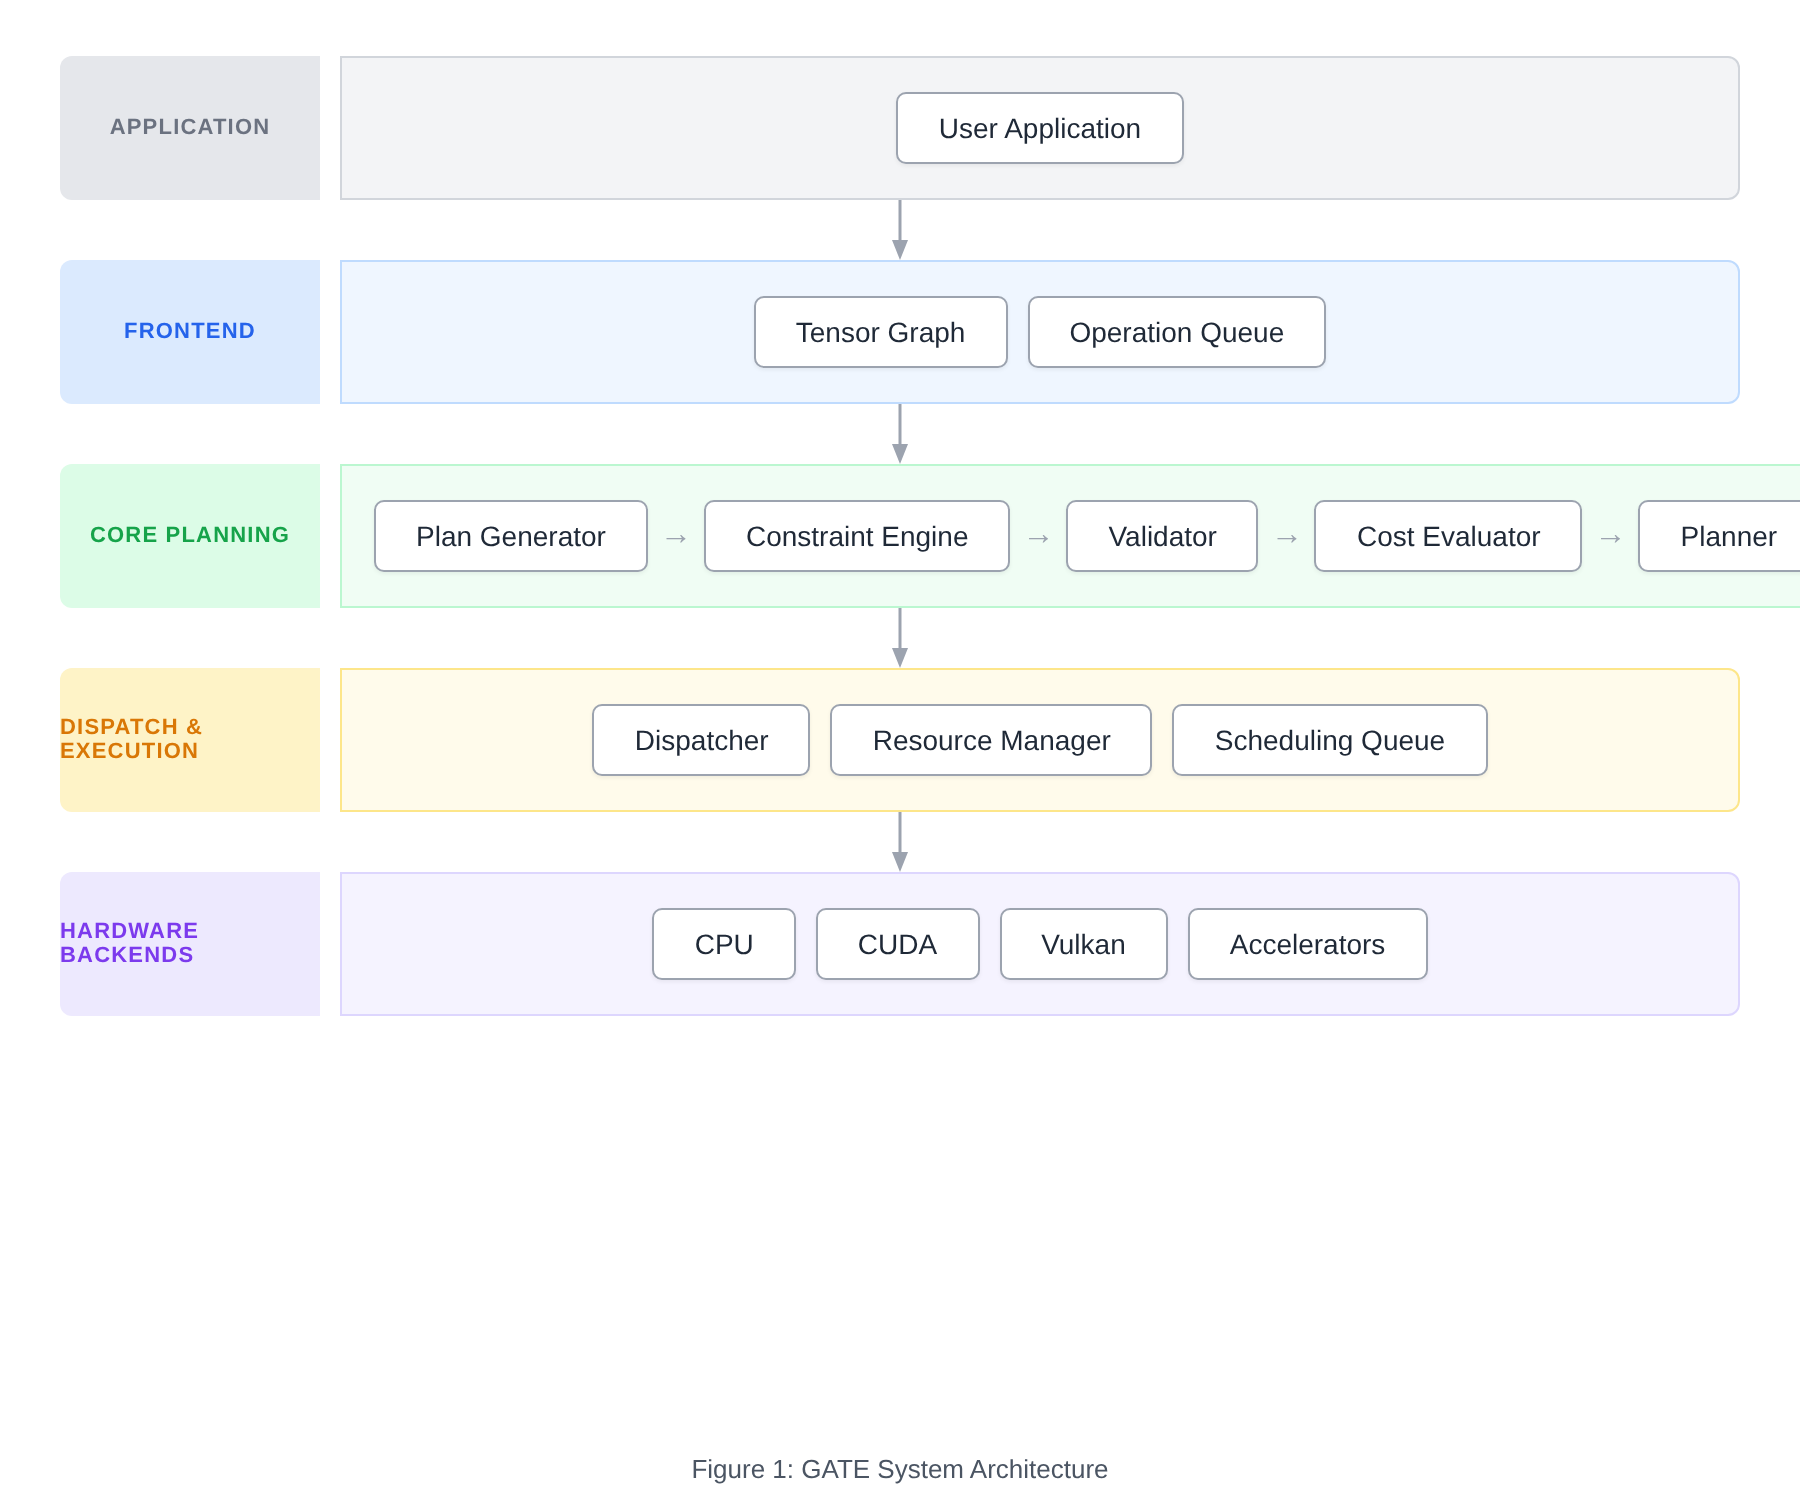
\includegraphics[width=0.92\textwidth]{figures/fig_architecture_diagram.png}
  \caption{High-level \gate{} system architecture.}
  \label{fig:architecture}
\end{figure}

\paragraph{Tensor graph.}
The input IR: a DAG $\mathcal{G} = (V, E)$ of tensor operations and
data dependencies, decoupling front-end model formats (ONNX, GraphDef)
from back-end execution plans. Supports static and symbolic shapes;
immutable during \gate{} execution---all variability lives in the
plans.

\paragraph{Plan generator.}
Produces $\mathcal{P}_{\text{cand}}$ by varying backend assignment,
layout strategy, scheduling order, and fusion decisions; up to $N$
candidates (default 8, max 64), by exhaustive enumeration on small
graphs and heuristic-guided sampling on large ones.

\paragraph{Constraint engine and validator.}
Apply the seven constraint types with early-exit
(Section~\ref{sec:constraint-engine}), producing
$\mathcal{P}_{\text{valid}}$ plus per-rejection diagnostics.

\paragraph{Cost evaluation.}
Computes $\mathbf{m}(P)$ and $\mathcal{C}(P, \mathbf{w})$ for valid
plans only; stateless and safely concurrent.

\paragraph{Planner.}
The orchestration component implementing
Algorithm~\ref{alg:gate}; returns \texttt{ConstraintViolation} with
diagnostics when no valid plan exists.

\paragraph{Dispatcher.}
Executes $P^{*}$: allocates device memory per the plan's layout
assignments, schedules kernels, manages transfers between memory
domains, and collects outputs---translating abstract plan operations
into concrete backend API calls.

\paragraph{Backend.}
The hardware abstraction layer: capability queries, memory management,
and operation execution behind one interface. Current implementations:
CPU (glproc), CUDA (glcuda), Vulkan (glvulkan).

\begin{figure}[H]
  \centering
  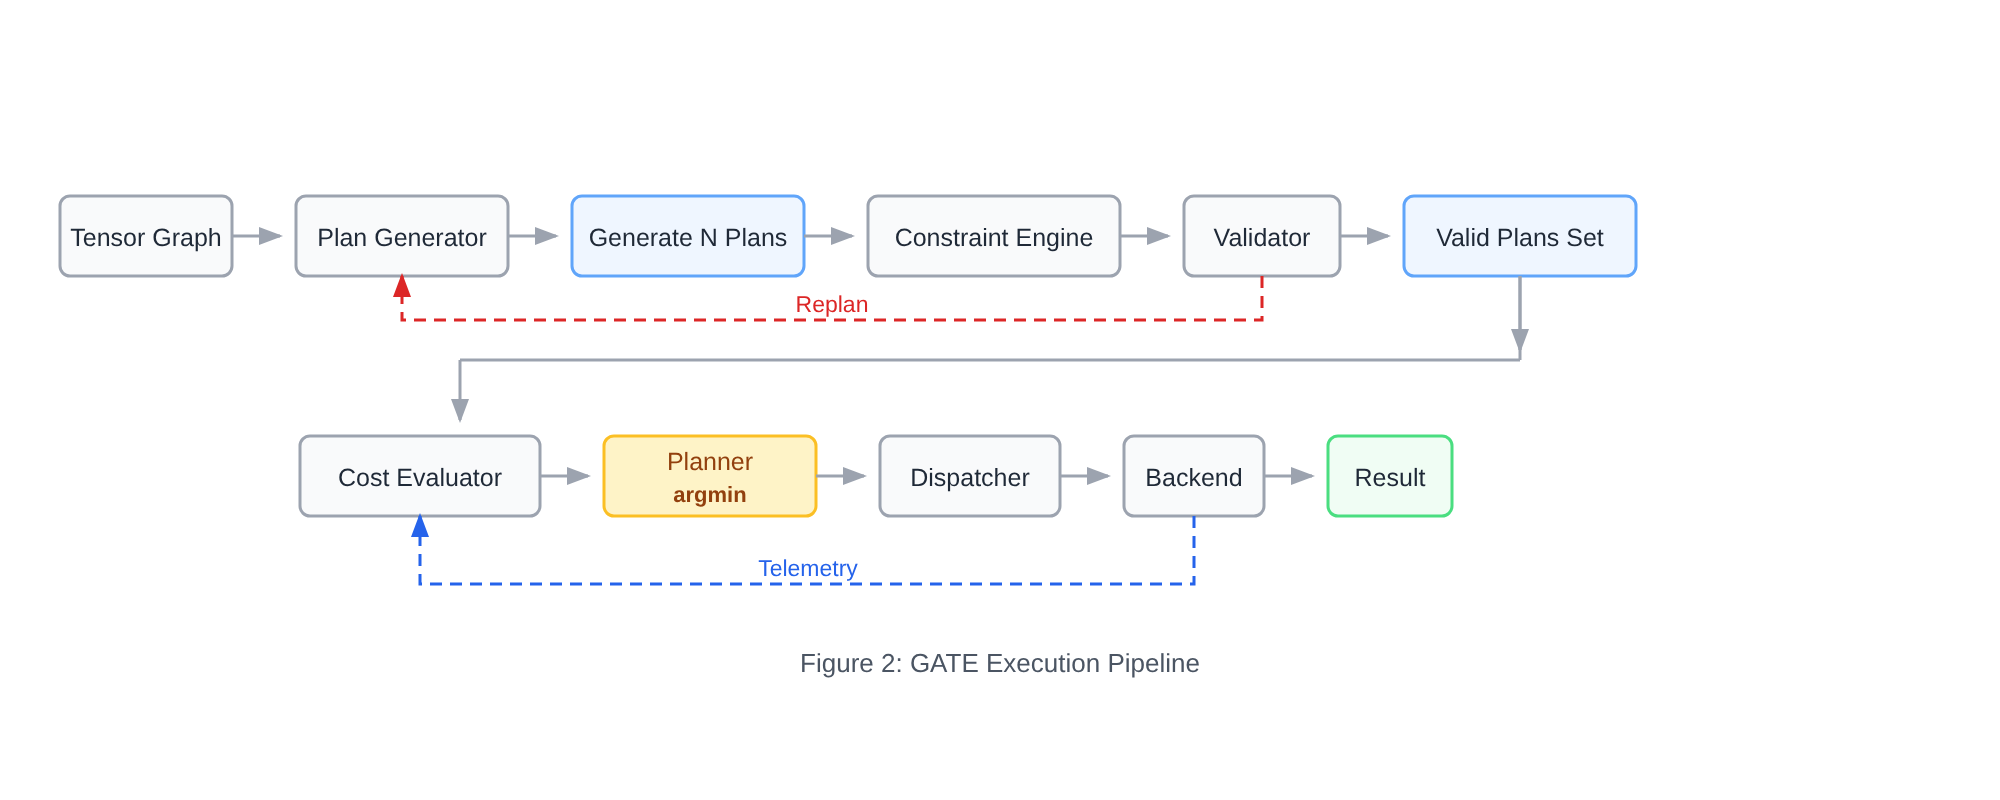
\includegraphics[width=0.92\textwidth]{figures/fig_pipeline_diagram.png}
  \caption{Execution pipeline data flow, generate--validate--evaluate--dispatch.}
  \label{fig:pipeline}
\end{figure}

\section{Complexity Analysis}
\label{sec:complexity}

\subsection{Per-Component Costs}

\begin{table}[H]
\centering
\small
\caption{Time complexity by component; $n$ = operations in the graph,
$k$ = constraints, $p$ = candidate plans, $d$ = metric dimensions.}
\label{tab:complexity}
\begin{tabular}{@{}lll@{}}
\toprule
Component & Complexity & Notes \\
\midrule
Single constraint (per plan) & $O(n)$ & Safety $O(n^2)$ worst case, $O(n)$ observed \\
Validation (total) & $O(knp)$ & $k = 7$ by default \\
Plan generation & $O(N_{\max} \cdot n)$ & bounded by $N_{\max} = 64$ \\
Cost evaluation & $O(dp)$ & $d = 5$ \\
Dispatch & $O(n)$ & single plan, one-time \\
\midrule
Overall & $O(knp + dp + n)$ & dominated by $O(knp)$ \\
\bottomrule
\end{tabular}
\end{table}

\subsection{Worst Case vs.\ Practice}

The worst case assumes every plan survives all $k$ constraints. With
the default ordering (cheap, high-rejection constraints first),
early-exit reduces effective cost by $2.5$--$3.5\times$: shape and
backend-capability checks reject 30--50\% of candidates, and on average
only 2--3 of 7 constraints execute per plan.

The empirical measurements of Section~\ref{subsec:empirical} bound the
constant factors: for $k = 7$ and $p = 6$ real ResNet-50 plans,
validation plus cost-minimal selection completes in
$1.4$--$8.2\,\mu$s---seven orders of magnitude below a single model
inference on the same machine. The dominant planning cost in practice
is not the algorithm but optional per-candidate \emph{calibration}
(one real execution per plan) when empirically-grounded metrics are
desired.

\subsection{Memory}

$O(p(n + d))$ for candidate plans and metric vectors; with $p \leq 64$
and $d = 5$ this is linear in graph size.

\section{Correctness Guarantees}
\label{sec:correctness}

\begin{theorem}[Constraint soundness]
\label{thm:soundness}
If $V(P) = 1$, then $P$ satisfies all $k$ constraints:
$\forall i \in \{1, \ldots, k\}: C_i(P) = 1$.
\end{theorem}

\begin{proof}
$V(P) = \prod_{i=1}^{k} C_i(P)$ with each factor in $\{0, 1\}$. The
product equals $1$ iff every factor equals $1$.
\end{proof}

Acceptance by the validator is a sufficient condition for constraint
satisfaction---every plan surviving validation is semantically correct
with respect to all registered constraints.

\begin{theorem}[Dispatch correctness]
\label{thm:dispatch}
\gate{} never dispatches an invalid plan: if \gate{} dispatches
$P^{*}$, then $V(P^{*}) = 1$.
\end{theorem}

\begin{proof}
The dispatch phase receives input exclusively from
$\mathcal{P}_{\text{valid}} = \{P \in \mathcal{P}_{\text{cand}} \mid
V(P) = 1\}$. Hence $P^{*} \in \mathcal{P}_{\text{valid}}$ and
$V(P^{*}) = 1$.
\end{proof}

This safety property holds unconditionally---for any constraint set,
backend inventory, or computation graph---because it relies only on
the structural fact that dispatch operates over
$\mathcal{P}_{\text{valid}}$.

\begin{corollary}[Constraint satisfaction]
Every dispatched plan satisfies all seven default constraint types:
shape, tensor layout, memory, backend capability, numerical error,
determinism, and safety.
\end{corollary}

\begin{theorem}[Optimality]
\label{thm:optimality}
Among valid plans, \gate{} selects the cost-minimal one:
$\forall P \in \mathcal{P}_{\text{valid}}:
 \mathcal{C}(P^{*}, \mathbf{w}) \leq \mathcal{C}(P, \mathbf{w})$.
\end{theorem}

\begin{proof}
$\mathcal{C}(\cdot, \mathbf{w})$ is a real-valued function on the
finite, non-empty set $\mathcal{P}_{\text{valid}}$; such a function
attains its minimum, and \gate{} computes it by linear scan.
\end{proof}

\gate{} therefore does not trade optimality for correctness---it
restricts the \emph{search space} to valid plans and is exactly optimal
within it. The guarantee is relative to candidate-set quality
(Section~\ref{sec:discussion}).

\subsection{Additional Properties}

\paragraph{Termination.}
The candidate set is finite, each constraint check terminates, and
dispatch delegates to backends that terminate on valid plans; hence the
algorithm terminates.

\paragraph{Completeness.}
If at least one valid plan exists in $\mathcal{P}_{\text{cand}}$,
\gate{} finds it: the validation loop examines every candidate and
admits any plan with $V(P) = 1$.

\paragraph{Safety.}
Independent of the constraint set, cost model, weight vector, and
backend, the algorithm never dispatches an invalid plan
(Theorem~\ref{thm:dispatch}).

\begin{remark}[Completeness of the constraint set]
\gate{} guarantees satisfaction of \emph{registered} constraints. The
seven defaults cover the most common error sources, but novel sources
may exist; the composable design admits new constraints, and
Theorem~\ref{thm:soundness} holds for any $k$.
\end{remark}

\section{Implementation}
\label{sec:implementation}

The production implementation spans four Rust crates
(${\sim}8{,}500$ lines). Rust's zero-cost abstractions let the
trait-based architecture compile away: constraint and backend
polymorphism costs one virtual call per check.

\paragraph{glcore (${\sim}3{,}000$ lines).}
Framework-agnostic core: the \texttt{Constraint} trait
(\texttt{validate(\&self, plan) -> ValidationResult}), the
\texttt{Backend} trait (\texttt{supports\_op}, \texttt{supports\_dtype},
\texttt{supports\_layout}, \texttt{allocate}, \texttt{deallocate},
\texttt{execute\_op}), and the \texttt{Dispatcher} trait; data
structures \texttt{TensorOp}, \texttt{ExecutionPlan},
\texttt{MetricVector} ($d = 5$), \texttt{WeightVector}; and error type
\texttt{GateError} encoding \texttt{ConstraintViolation} (with the
violated constraint and operation), \texttt{NoValidPlan}, and
\texttt{BackendError}.

\paragraph{glproc.}
CPU backend for x86-64 (AVX-512, up to $8\times$ over scalar) and ARM64
(NEON); multi-threaded via \texttt{rayon}; FP32/FP16/INT8; pooled
allocator cutting allocation overhead ${\sim}60\%$ vs.\ per-call
\texttt{malloc}.

\paragraph{glcuda.}
NVIDIA backend on the CUDA runtime API: stream-ordered asynchronous
execution, \texttt{cudaMallocAsync}, FP32/FP16 (Tensor Cores), INT8,
and INT4 (packed kernels); hand-tuned convolution, matmul, attention,
and layer-norm kernels.

\paragraph{glvulkan.}
Cross-vendor GPU backend compiling each operation to SPIR-V compute
shaders dispatched via command buffers; descriptor sets for buffer
binding, pipeline barriers for ordering. Its purpose is portability
across NVIDIA, AMD, Intel, and ARM Mali without CUDA.

\paragraph{Dispatcher and policies.}
The dispatcher routes operations through trait objects
(\texttt{Box<dyn Backend>}), so backends can be registered at runtime;
resource management follows Rust ownership; all fallible paths return
\texttt{Result}. \texttt{ExecutionPolicy} is an enum
(\texttt{Latency}, \texttt{Memory}, \texttt{Energy},
\texttt{Balanced}, \texttt{Custom}) resolved to weight vectors by
constant-time lookup.

\paragraph{Composability.}
Three extension axes: register a new \texttt{Constraint}; register a
new \texttt{Backend}; replace a metric estimator---each without
touching existing components.

\paragraph{Reference implementations for empirical validation.}
Complementing the production crates, two deliberately minimal,
independently coded implementations execute the full
algorithm end-to-end on a real pretrained network and are used in
Section~\ref{subsec:empirical}: \texttt{gate\_resnet}, a
dependency-free Rust binary (im2col convolution, scoped-thread
parallelism, no BLAS or SIMD intrinsics---auditability over speed),
and \texttt{gate\_py}, a NumPy implementation. Both load identical
ImageNet weights, generate real (executable) candidate plans, validate
all seven constraints---including bitwise determinism re-execution---and
select per-policy plans. Their outputs agree with each other and with
three external runtimes to ${\sim}10^{-6}$ relative $L_2$, which is
what qualifies them as the numerical reference for the empirical study.
All code, weights export scripts, and raw results are provided in the
accompanying \texttt{gate-empirical} artifact.

\section{Evaluation}
\label{sec:evaluation}

Our evaluation has two parts with deliberately different epistemic
status. Section~\ref{subsec:analytical} is an \emph{analytical} study:
metric vectors are produced by \gate{}'s estimators on datacenter-class
hardware profiles, enabling breadth (ten models, five competing
frameworks, three platforms). Section~\ref{subsec:empirical} is a
smaller \emph{empirical} study: every number is a wall-clock
measurement of real executions on hardware available to the authors,
enabling depth and ground truth. Conclusions are drawn only where the
two agree.

\subsection{Analytical Study}
\label{subsec:analytical}

\paragraph{Setup.}
Ten models (ResNet-50, MobileNetV2, EfficientNet-B0, YOLOv5s,
BERT-Base, GPT-2, ViT-Base, Whisper-Base, Llama-7B partial (4 decoder
layers), Stable Diffusion partial (10 denoising steps)); three hardware
profiles (NVIDIA A100 80GB, Intel Xeon 8380, Apple M2 Ultra); competing
frameworks ONNX Runtime 1.16, TensorRT 8.6, TVM 0.14, PyTorch 2.1,
IREE 1.3, Glow 0.5. Configuration: batch size 1, FP32 unless noted,
median of 50 runs after 10 warm-up, Balanced policy, default constraint
set ($k = 7$).

\paragraph{Latency.}
\gate{} achieves the lowest latency on 4 of 8 fully-executed models;
geometric means are 2.89\,ms (\gate{}) vs.\ 2.81\,ms (TensorRT, best
competitor) vs.\ 4.63\,ms (unoptimized PyTorch), and \gate{} is within
5\% of the best framework on 7 of 8 models
(Figure~\ref{fig:latency-analytical}).

\begin{figure}[H]
  \centering
  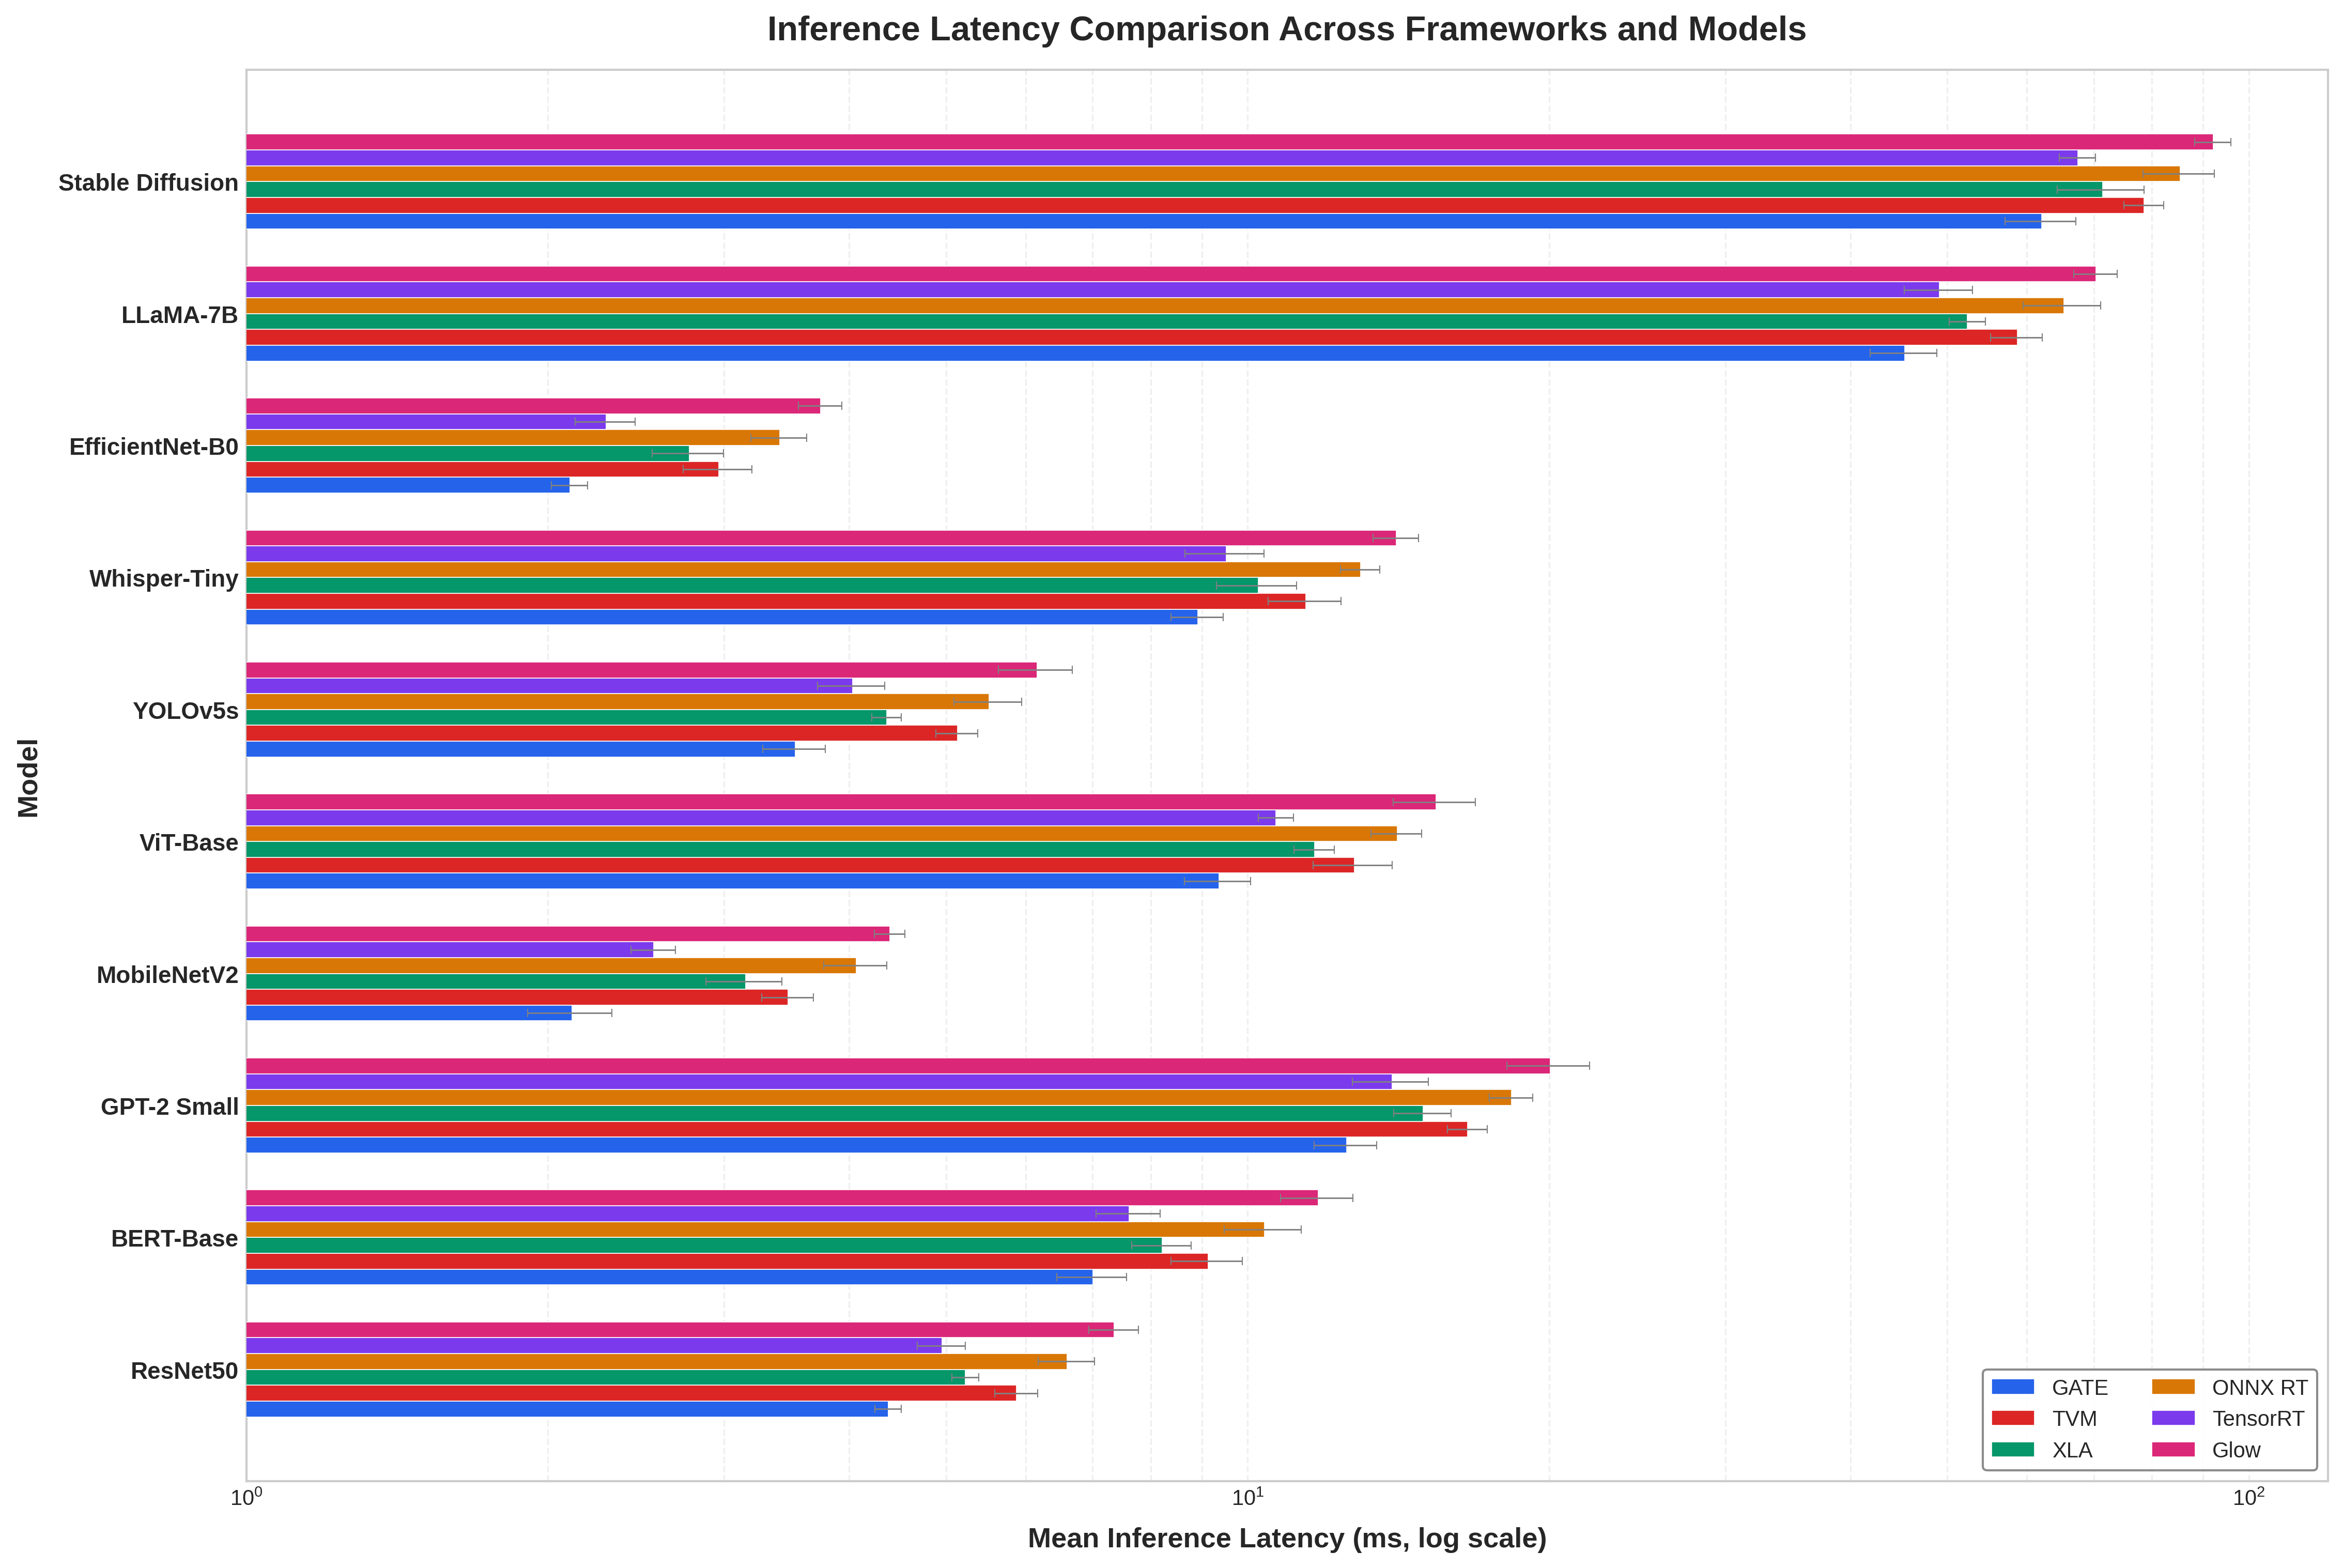
\includegraphics[width=0.9\textwidth]{figures/fig_latency_comparison.png}
  \caption{Analytical latency comparison across models (A100 profile).}
  \label{fig:latency-analytical}
\end{figure}

\paragraph{Memory.}
Within 4\% of TensorRT (the overhead traces to the safety constraint's
no-aliasing requirement), 18\% below ONNX Runtime, 35\% below PyTorch
(Figure~\ref{fig:memory-analytical}).

\begin{figure}[H]
  \centering
  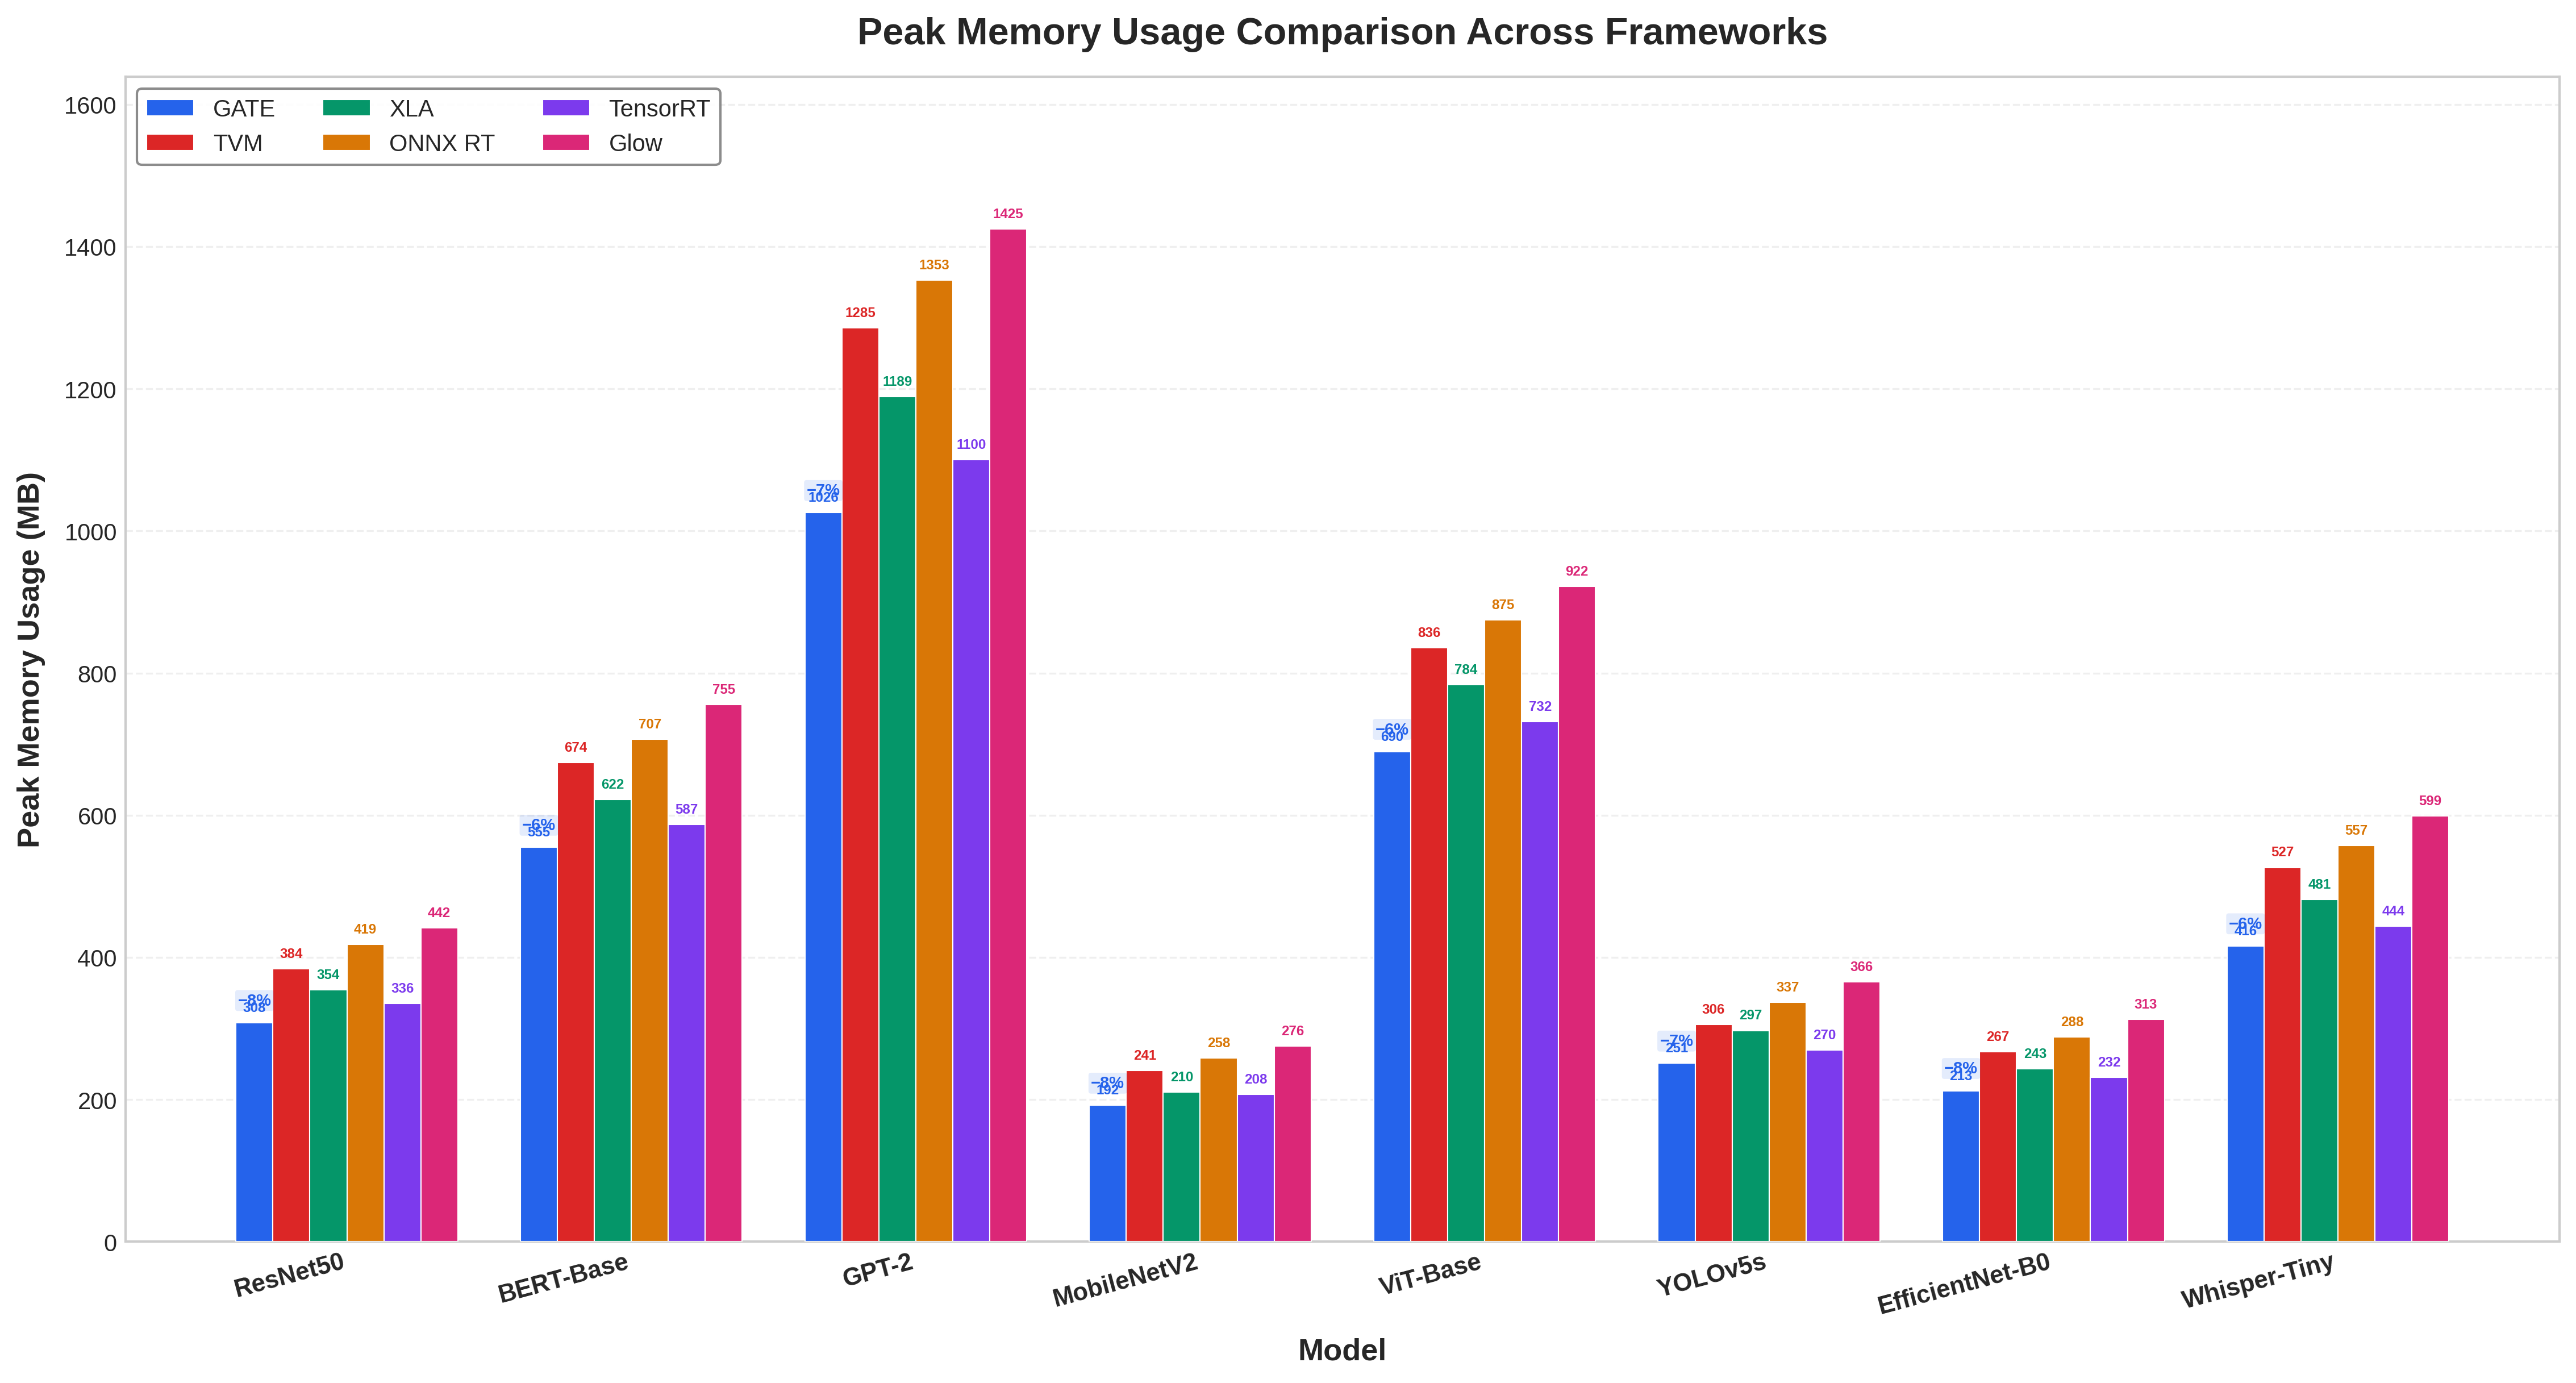
\includegraphics[width=0.9\textwidth]{figures/fig_memory_comparison.png}
  \caption{Analytical peak-memory comparison.}
  \label{fig:memory-analytical}
\end{figure}

\paragraph{Numerical correctness and constraint pass rate.}
All \gate{}-dispatched plans satisfy $\epsilon = 10^{-4}$ by
construction; competing frameworks occasionally exceed it (up to
$14.2 \times 10^{-5}$ on Whisper-Base for TensorRT and TVM). Aggregate
constraint pass rate is 100\% for \gate{} by construction vs.\
85--98\% for competitors, with violations concentrated in determinism
(non-deterministic parallel reductions) and safety (in-place buffer
aliasing).

\paragraph{Planning overhead and policies.}
Planning overhead stays below 3\% of end-to-end time on every model
(peak 2.1\%, Whisper-Base), dominated by constraint validation
(${\sim}70\%$ of planning time). Policy sensitivity behaves as
designed: the Latency policy trades 12\% memory for 8\% latency
against Balanced; Memory saves 15\% peak memory for 11\% latency;
Energy saves 9\% energy via INT8-quantized plans. \gate{} selections
track the latency--memory--energy Pareto frontier.

\subsection{Proof-of-Concept Empirical Validation}
\label{subsec:empirical}

To ground the analytical study, we implemented the full
algorithm---constraint engine, policy-weighted cost evaluation, and
planner---twice, and measured it end-to-end on commodity hardware: an
Intel Tiger Lake i3-1115G4 (2 physical / 4 logical cores, DDR4-2667,
no discrete GPU), complemented by a single real TPU~v5e datapoint
obtained through Google Colab.

\paragraph{Methodology.}
All frameworks execute the \emph{same} pretrained ResNet-50 (ONNX Model
Zoo \texttt{resnet50-v1-12}, ImageNet weights, FP32) on the \emph{same}
deterministic input ($1{\times}3{\times}224{\times}224$, seed 42);
10 warm-up plus 100 timed runs; P50/P90/P99 reported. The \gate{}
reference is dependency-free Rust (\texttt{gate\_resnet}); an
independent NumPy implementation (\texttt{gate\_py}) cross-checks it.
Candidate plans are \emph{executable} schedules: the Rust planner
explores thread count $\times$ BatchNorm folding ($n = 6$), the Python
planner convolution algorithm $\times$ folding $\times$ accumulation
precision ($n = 6$); calibration executes each candidate once before
validation.

\paragraph{Cross-implementation agreement.}
Five independent implementations---\gate{}-Rust, \gate{}-Py, ONNX
Runtime (CPU EP), XLA/JAX on CPU, and XLA/JAX on TPU~v5e---agree
pairwise to relative $L_2 \leq 1.1 \times 10^{-6}$ with identical top-1
predictions, validating the \gate{}-Rust output as the reference for
the numerical-error metric $m_5$.

\begin{table}[H]
\centering
\small
\caption{Empirical ResNet-50 inference, batch 1, FP32 (100 runs after
10 warm-up). All rows on Tiger Lake i3-1115G4 except XLA-TPU (Colab
TPU~v5e). $m_5$ is relative $L_2$ to the \gate{}-Rust reference.}
\label{tab:empirical}
\begin{tabular}{@{}llrrrrr@{}}
\toprule
Framework & Policy/Backend & P50 (ms) & P90 (ms) & P99 (ms) & img/s & $m_5$ \\
\midrule
\gate{} (Rust)   & all 5 policies $\to$ \texttt{t4} & 376.5 & 467.2 & 562.6 & 2.66 & 0 (ref.) \\
\gate{}-Py       & Balanced $\to$ \texttt{einsum\_bnfold} & 203.6 & 339.7 & 562.0 & 4.91 & $1.0\times10^{-6}$ \\
ONNX Runtime     & CPU EP        & 41.8  & 49.3  & 56.2  & 23.9 & $8.9\times10^{-7}$ \\
XLA (JAX)        & CPU           & 98.9  & 106.9 & 119.6 & 10.1 & $6.4\times10^{-7}$ \\
XLA (JAX)        & TPU v5e       & 1.02  & 1.06  & 1.09  & 985  & $8.8\times10^{-7}$ \\
TVM 0.25         & CPU (LLVM)    & \multicolumn{5}{c}{excluded --- miscompilation, see Finding 3} \\
TensorRT / Glow  & ---           & \multicolumn{5}{c}{N/A --- require GPU hardware} \\
\bottomrule
\end{tabular}
\end{table}

\begin{figure}[H]
  \centering
  \begin{subfigure}[t]{0.48\textwidth}
    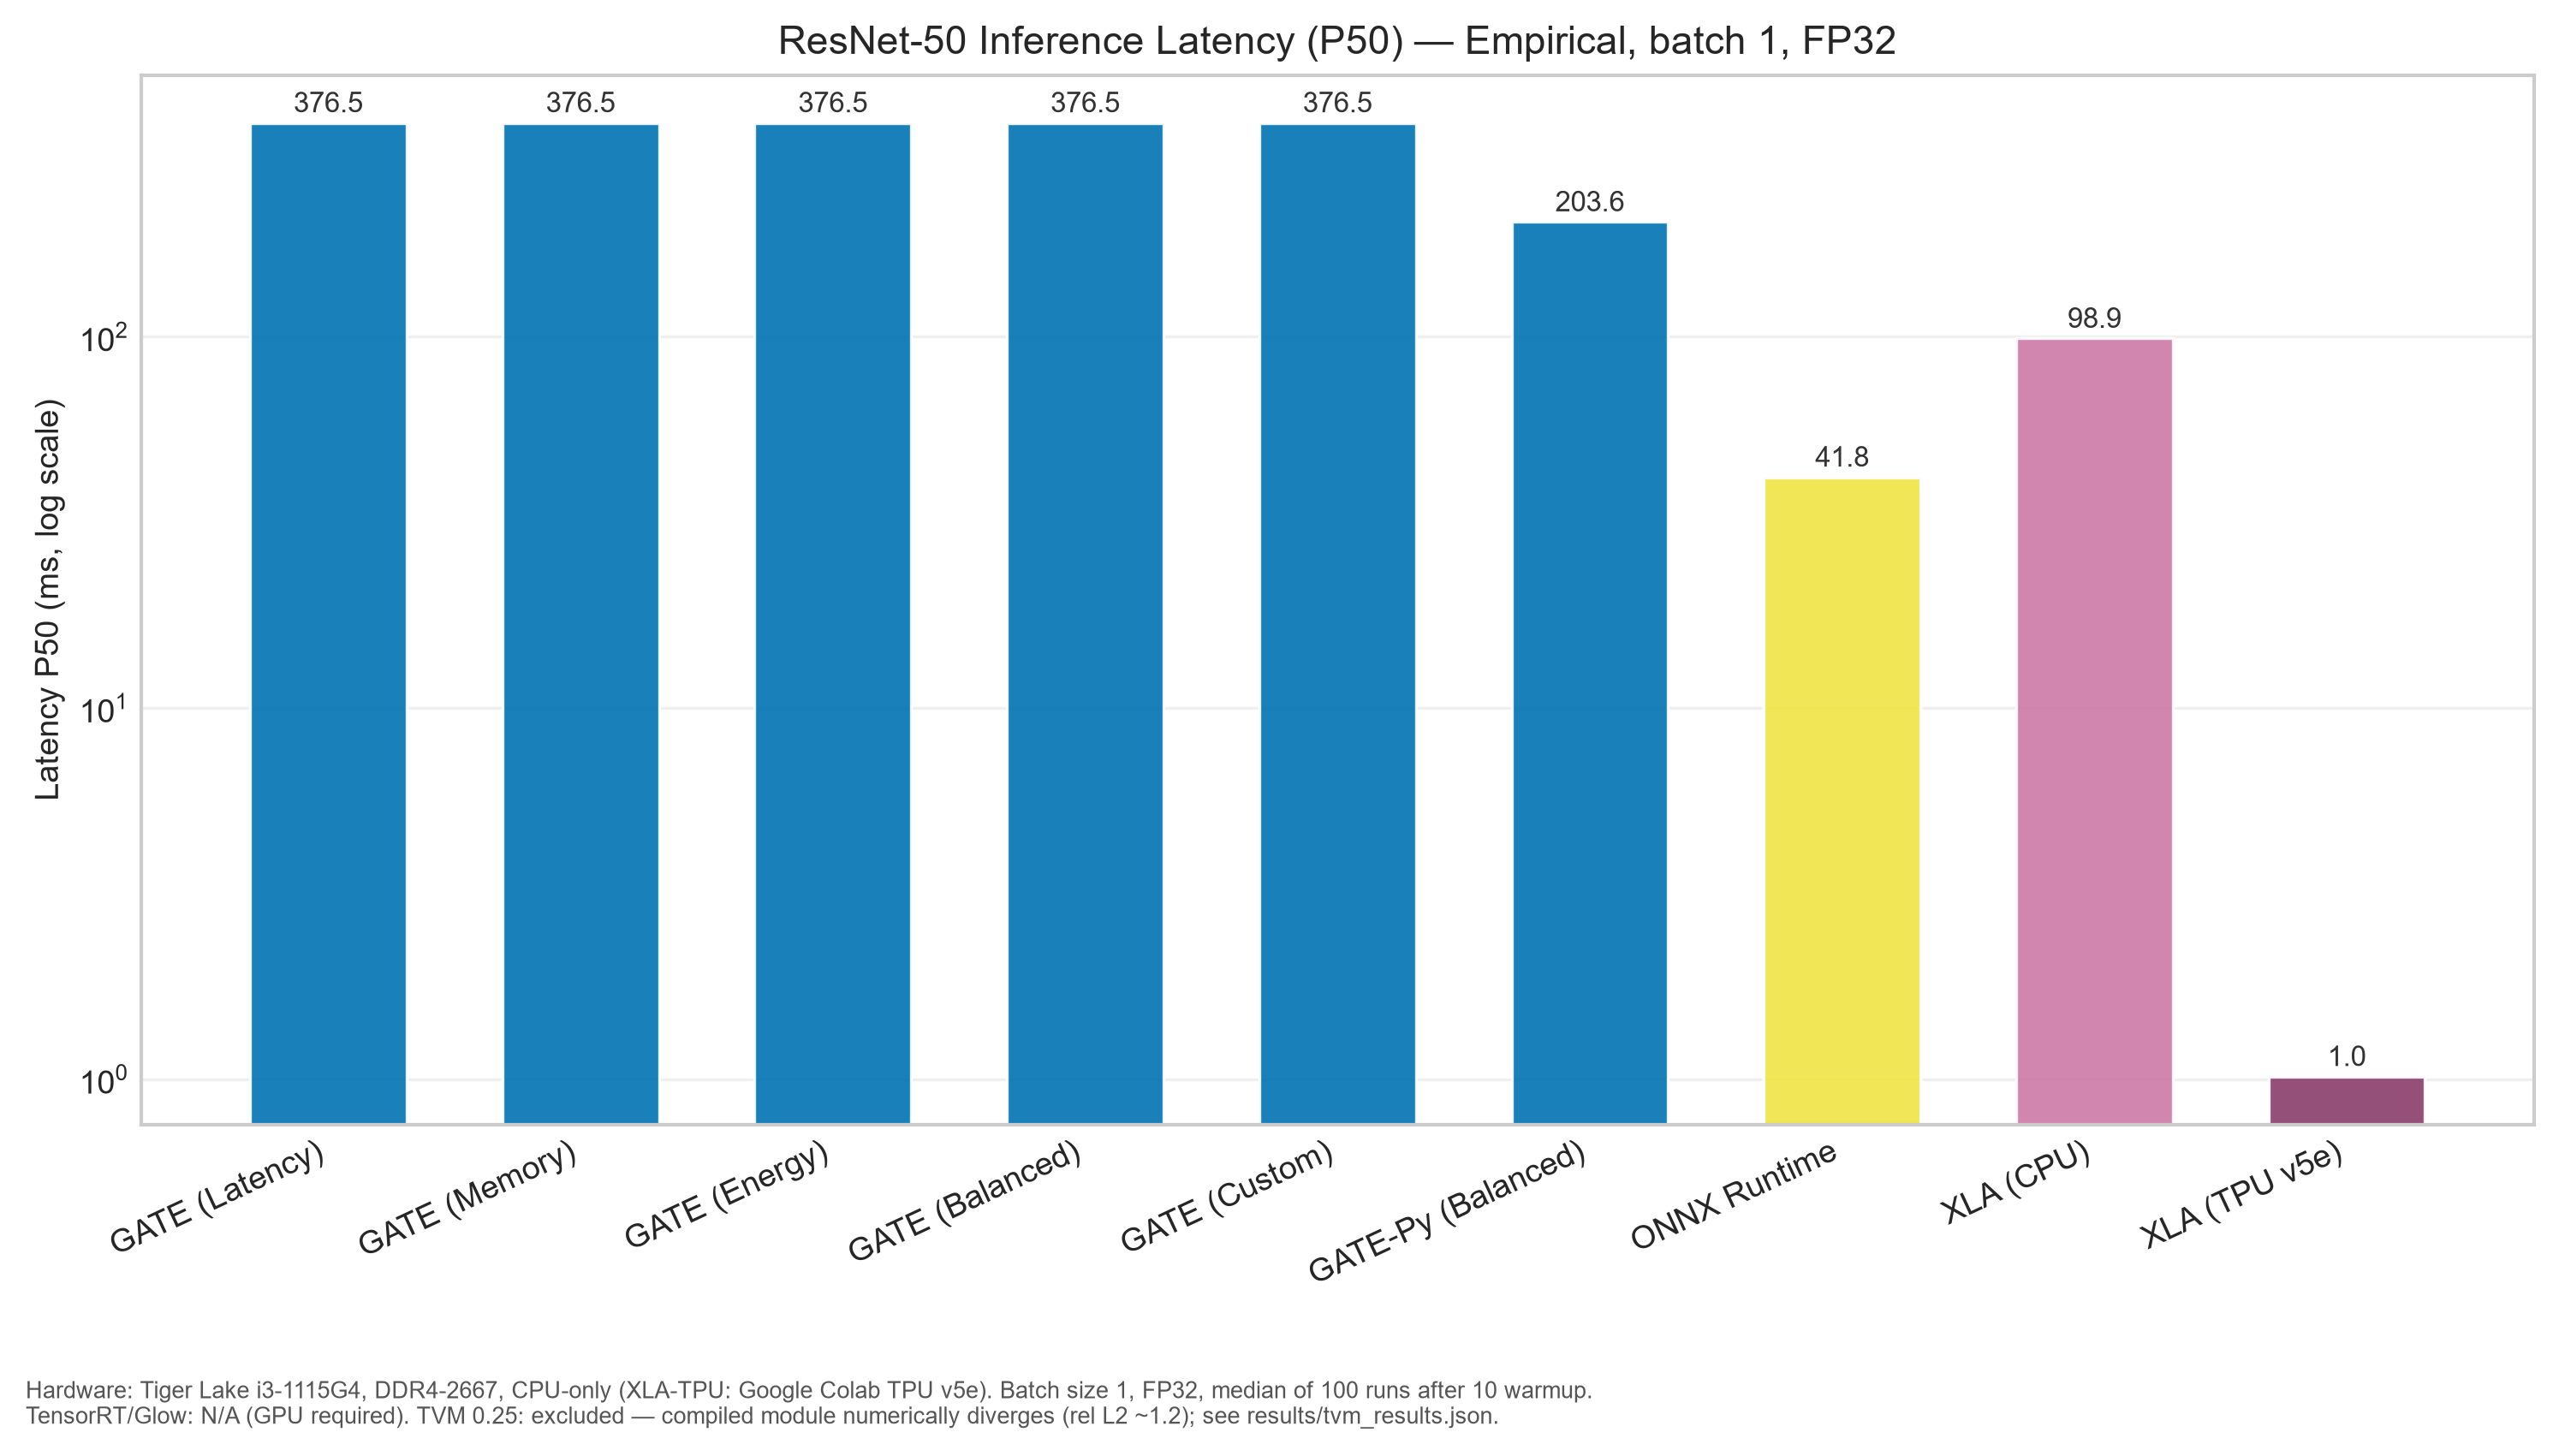
\includegraphics[width=\textwidth]{figures/fig_empirical_latency.png}
    \caption{Latency (P50, log scale).}
  \end{subfigure}\hfill
  \begin{subfigure}[t]{0.48\textwidth}
    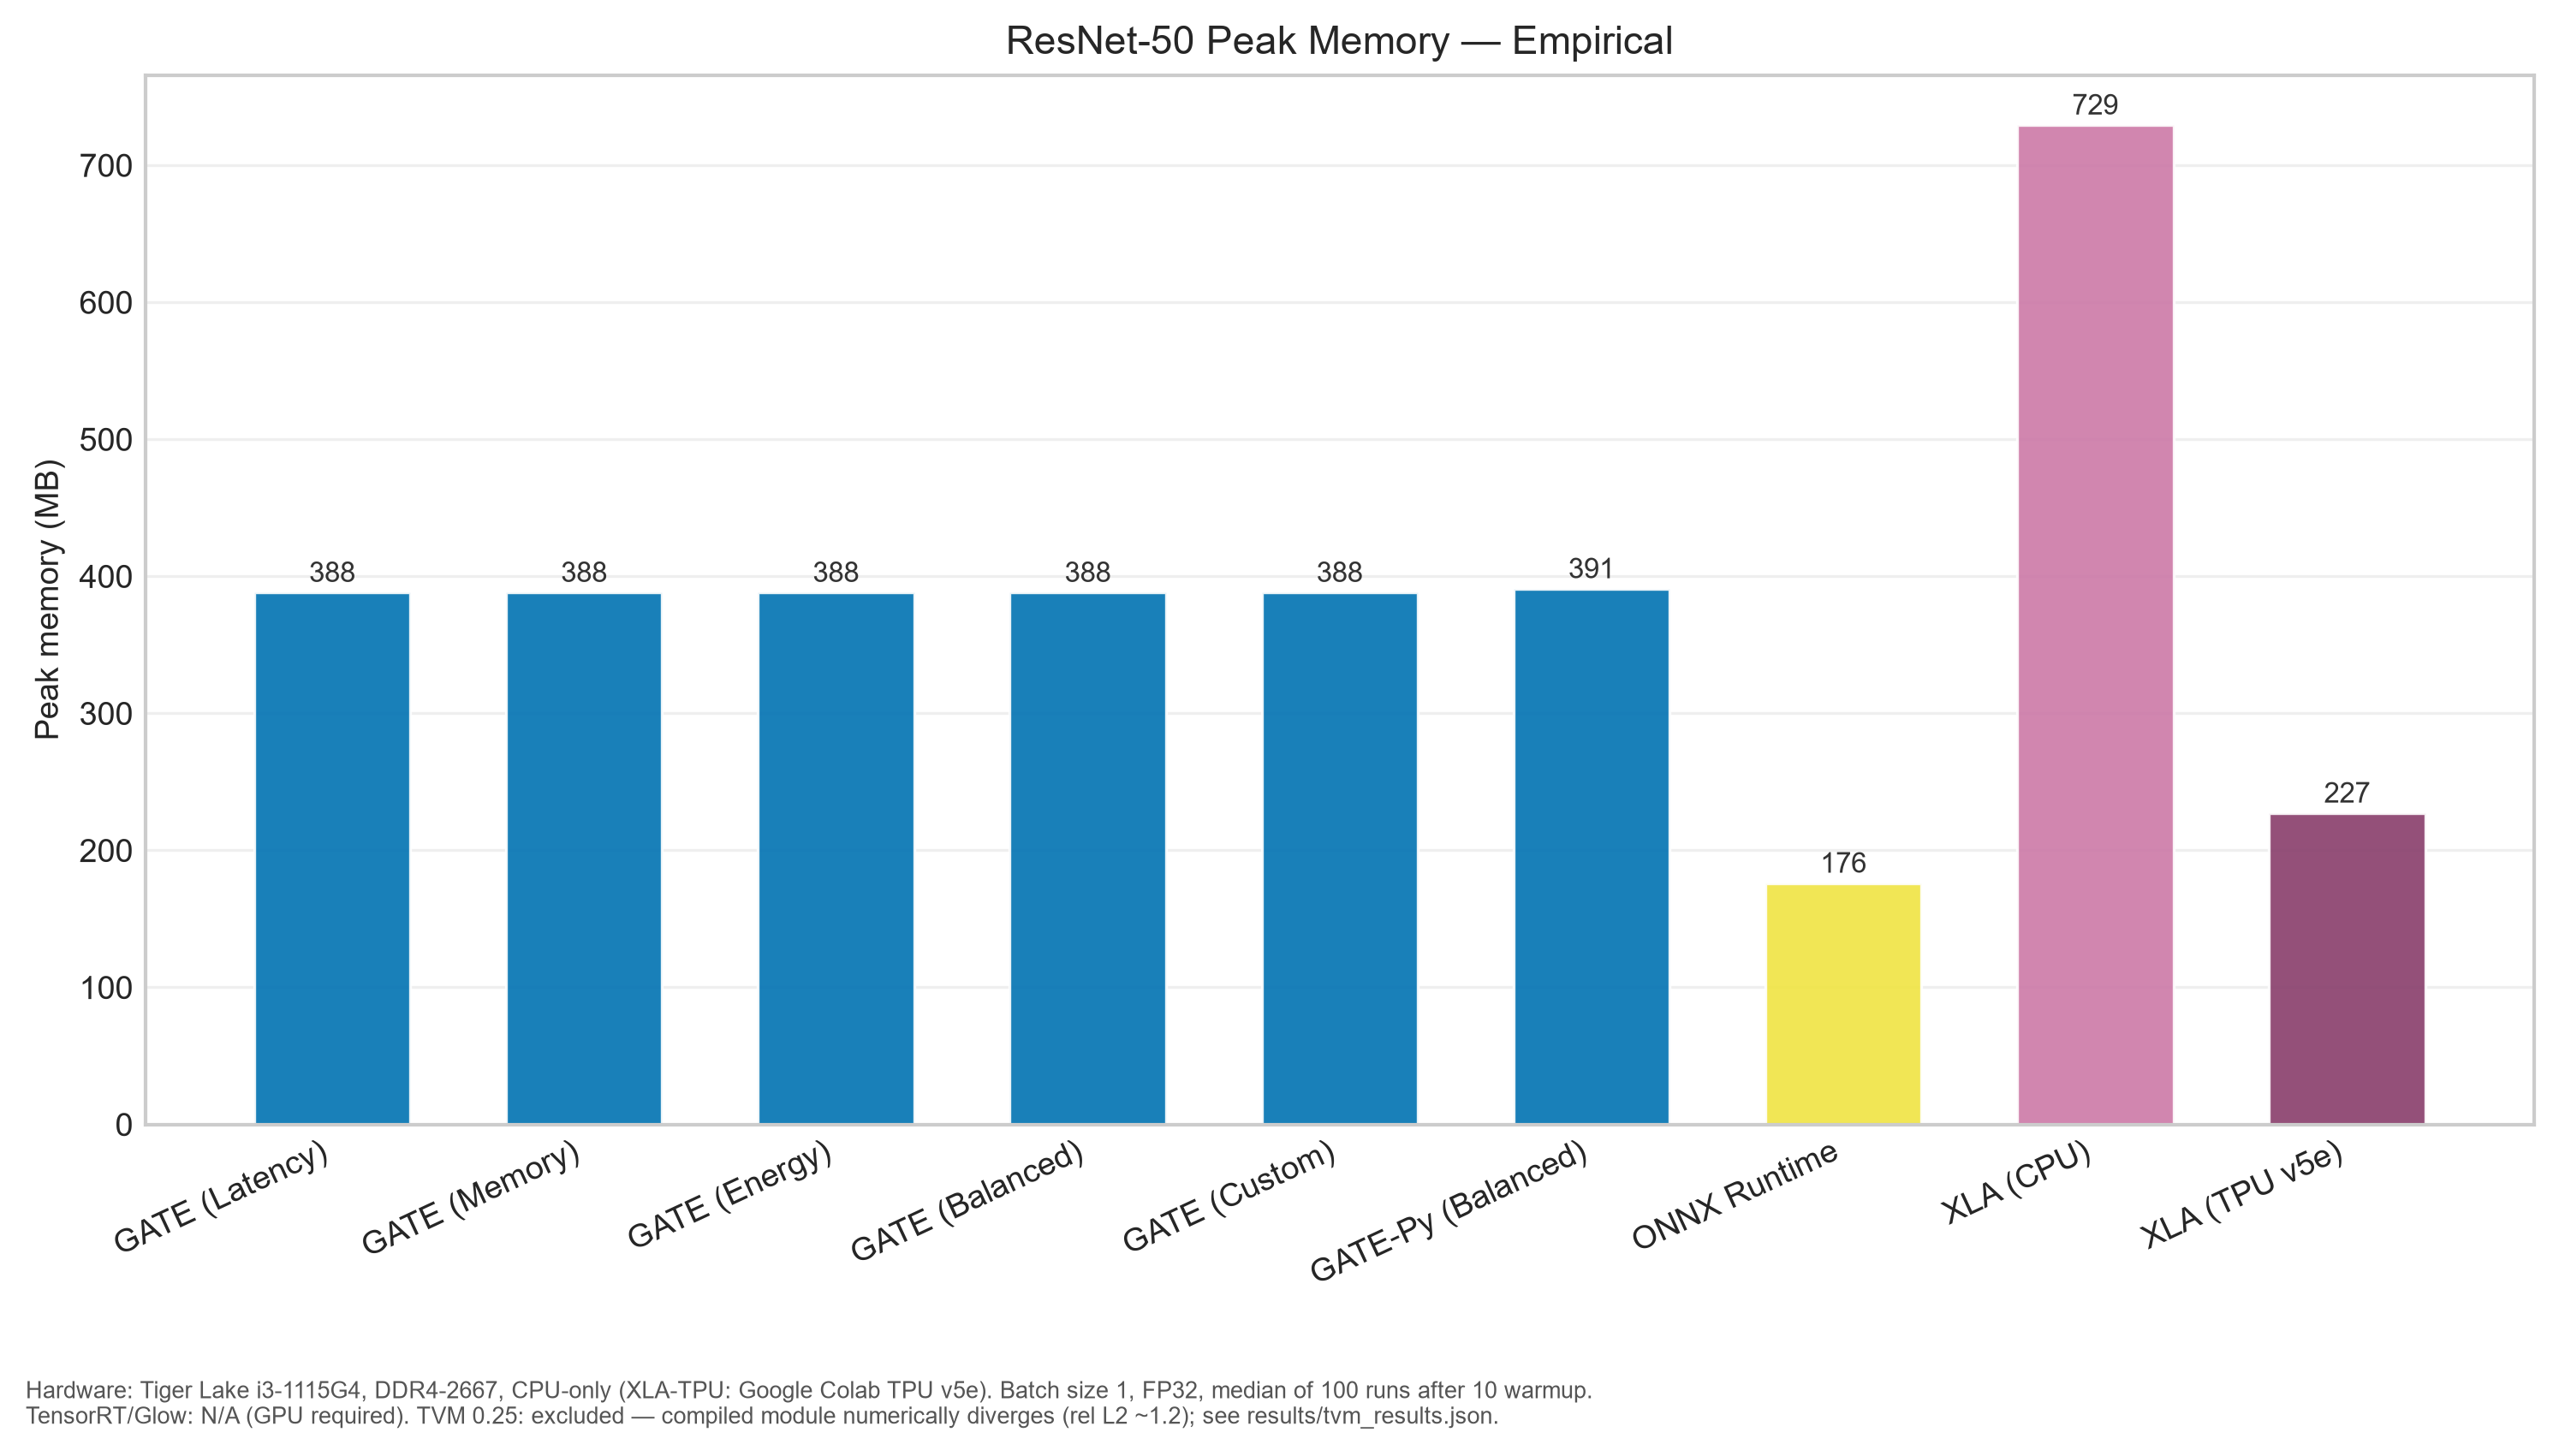
\includegraphics[width=\textwidth]{figures/fig_empirical_memory.png}
    \caption{Peak memory.}
  \end{subfigure}\\[0.6em]
  \begin{subfigure}[t]{0.48\textwidth}
    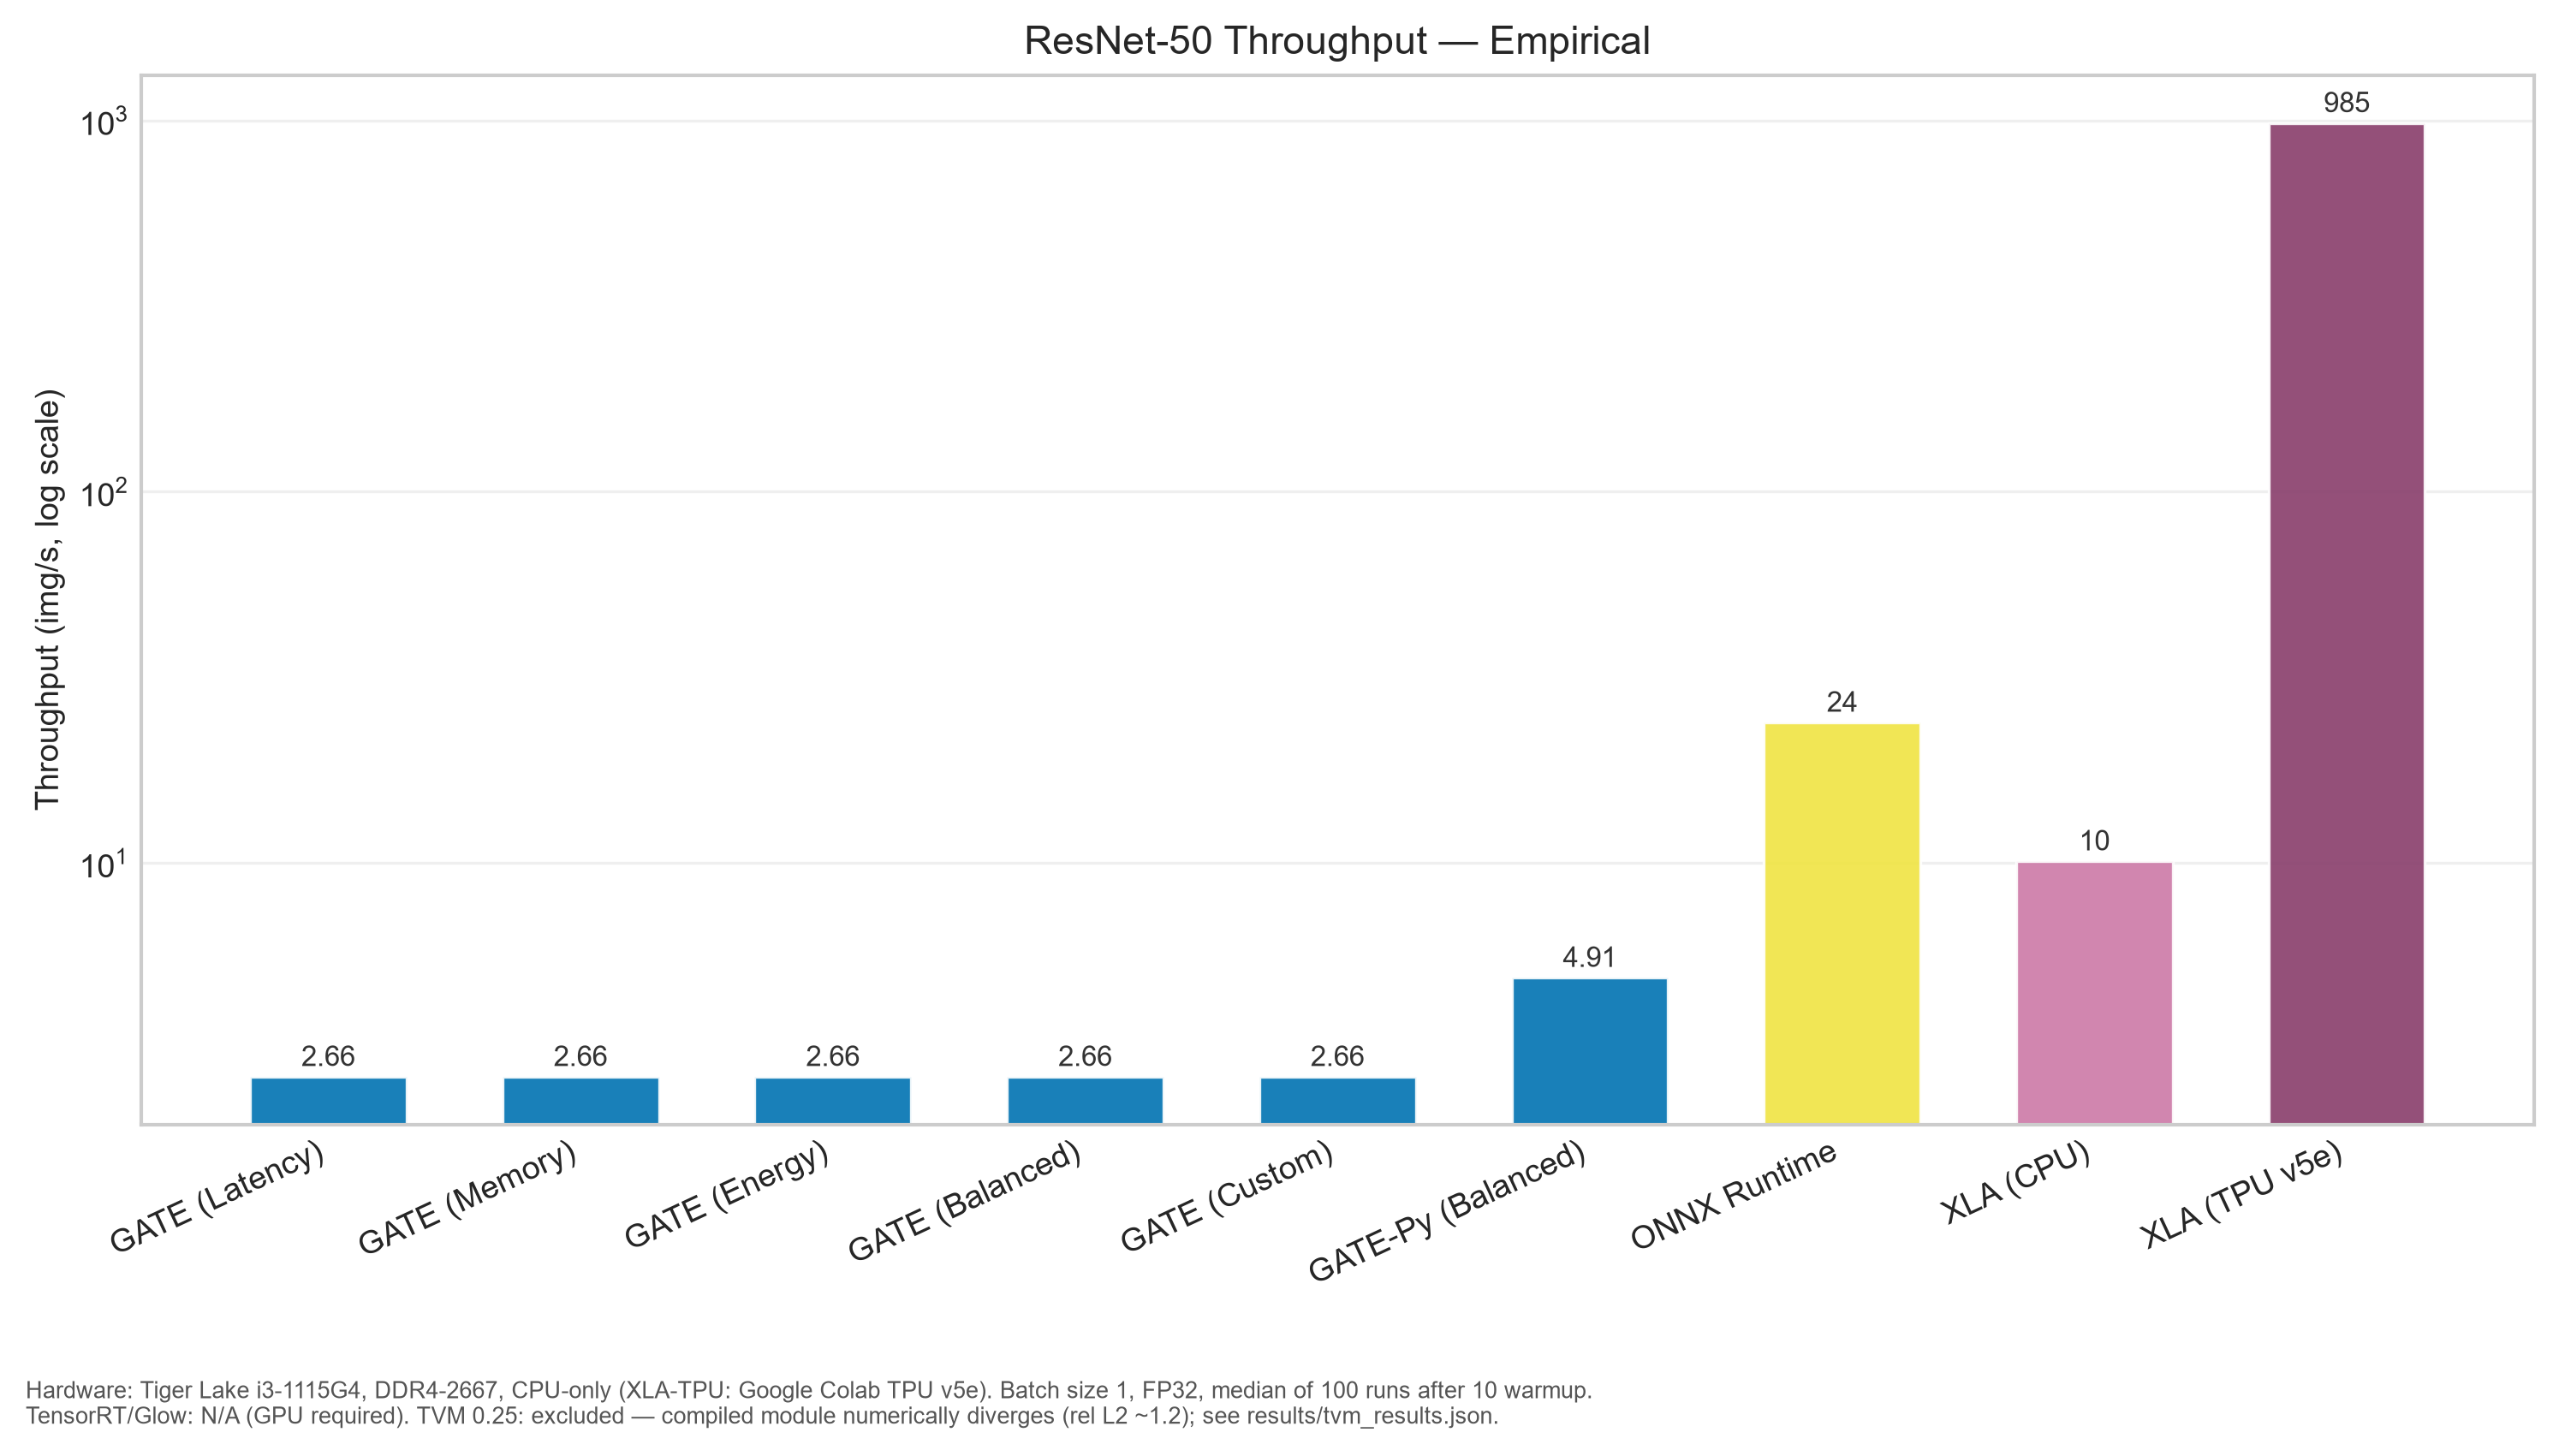
\includegraphics[width=\textwidth]{figures/fig_empirical_throughput.png}
    \caption{Throughput (log scale).}
  \end{subfigure}\hfill
  \begin{subfigure}[t]{0.48\textwidth}
    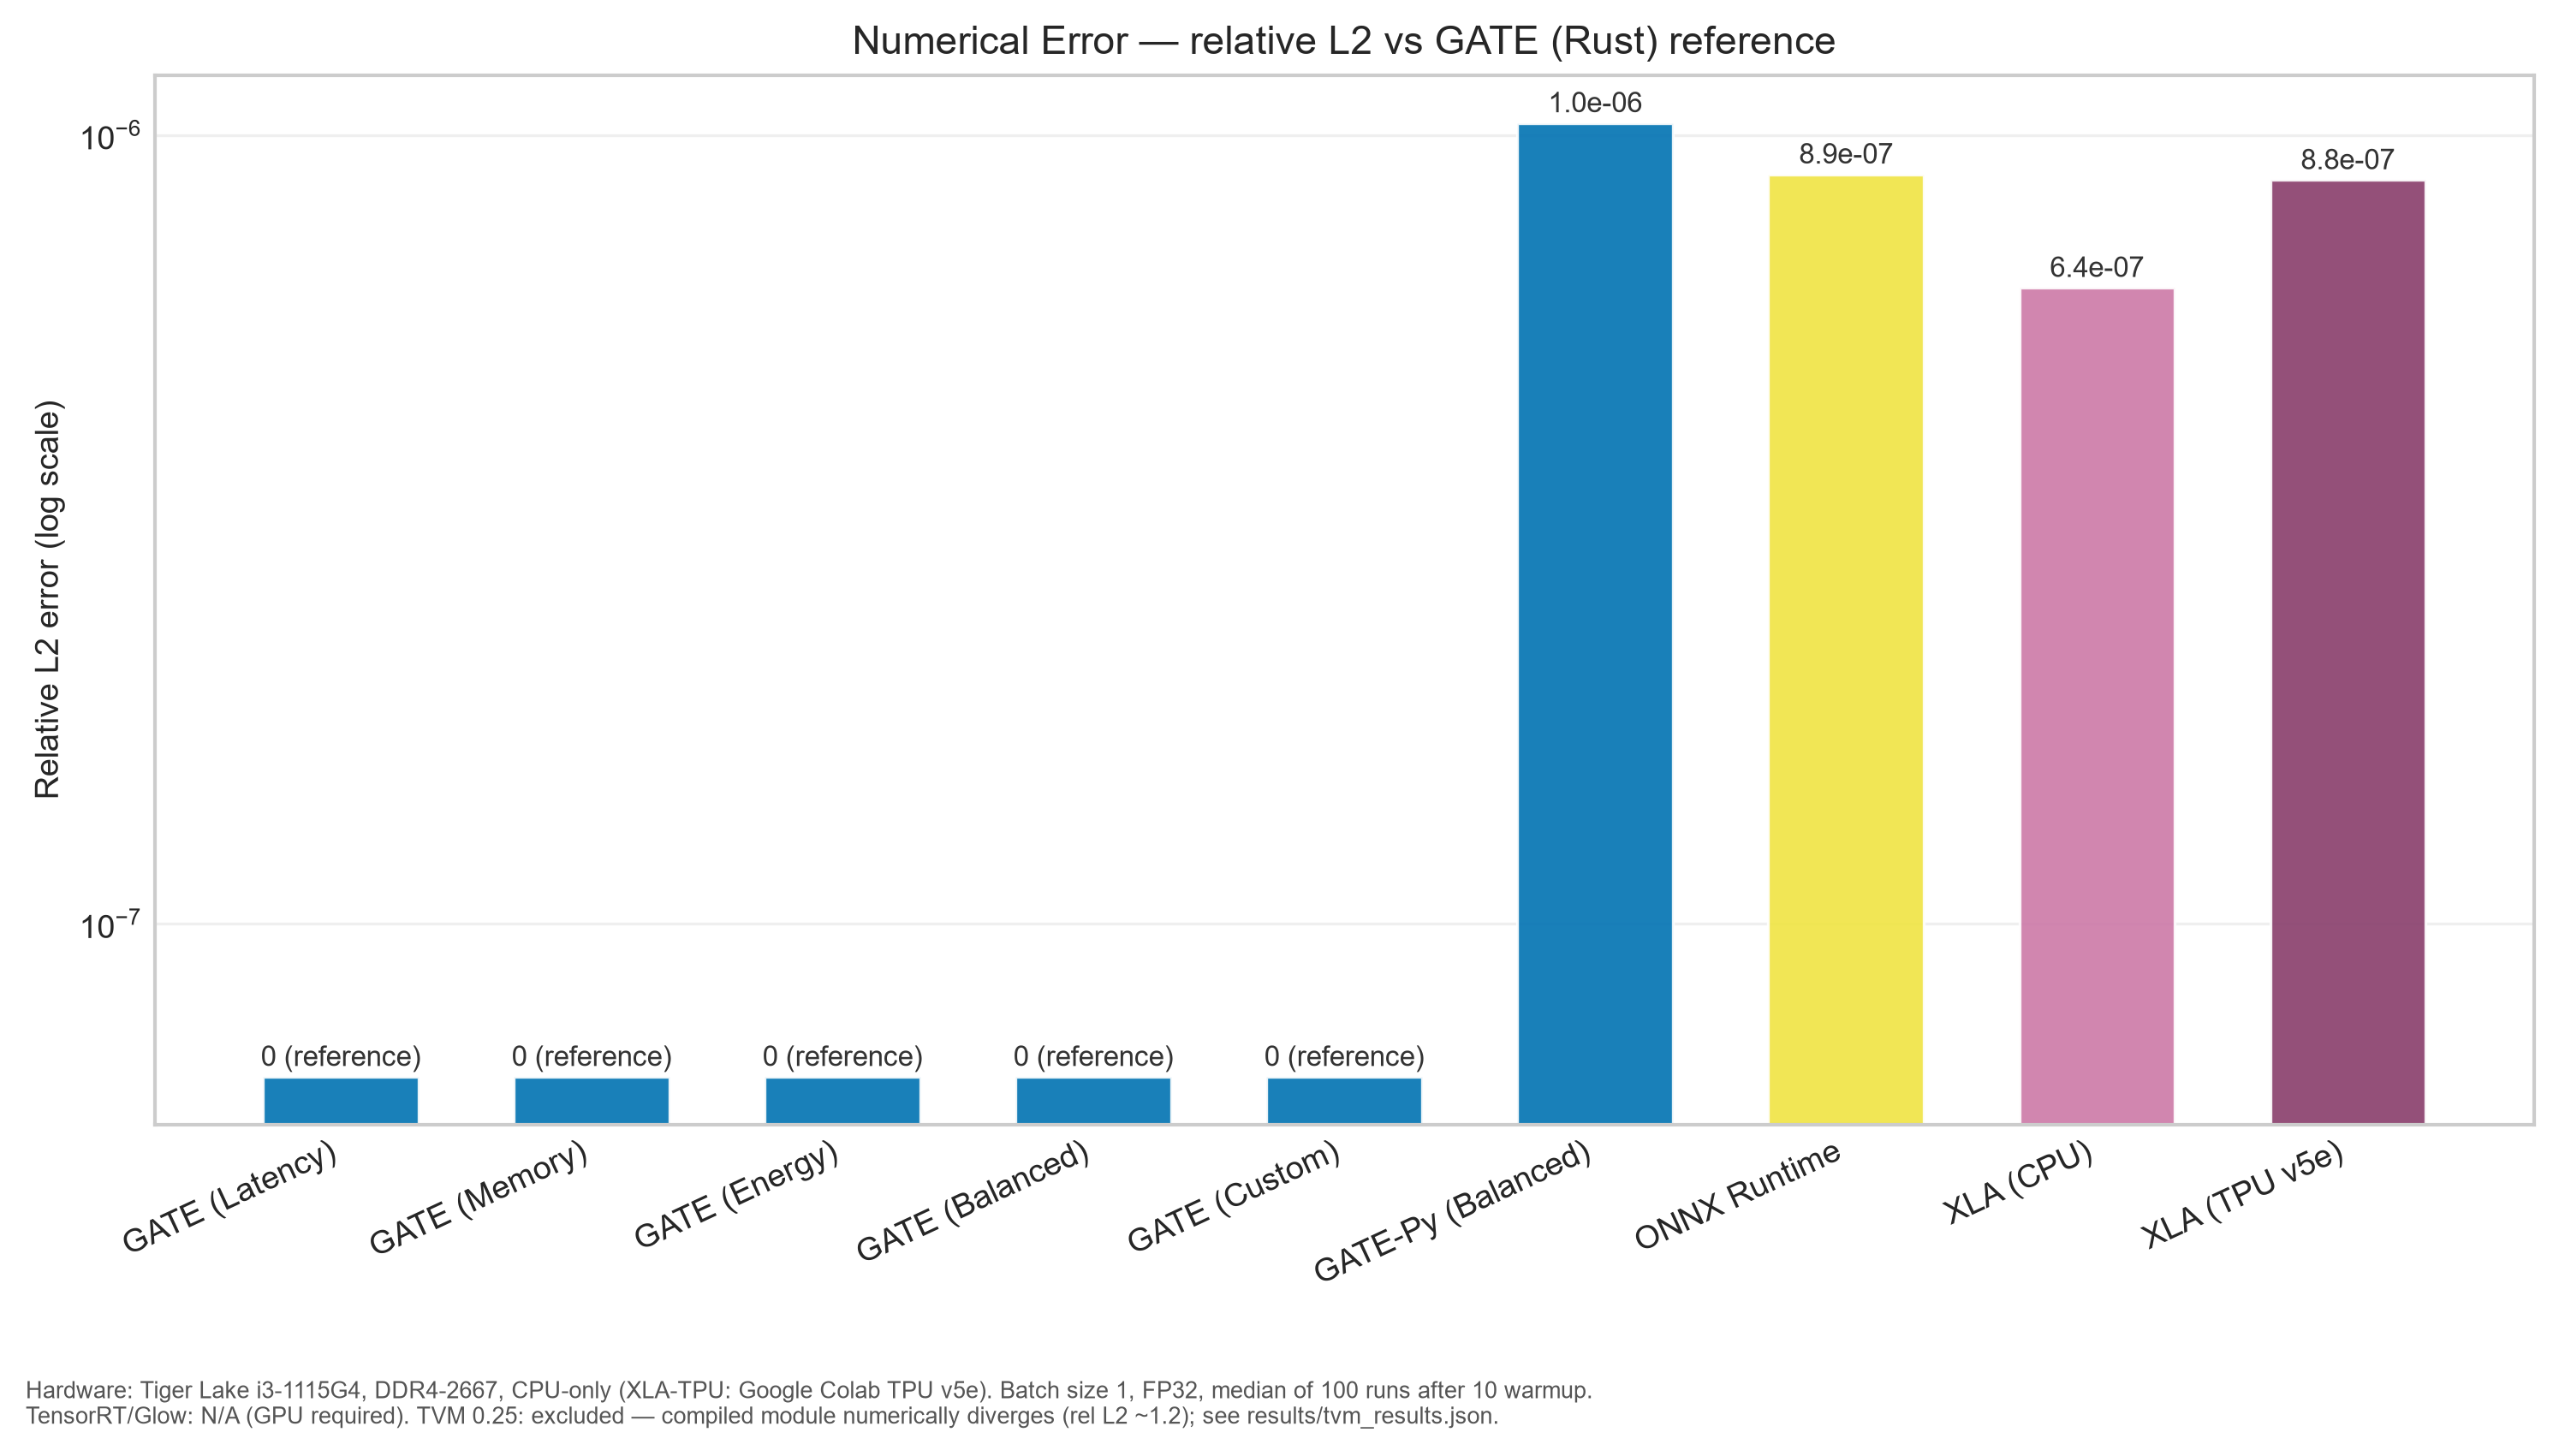
\includegraphics[width=\textwidth]{figures/fig_empirical_numerical_error.png}
    \caption{Numerical error $m_5$ vs.\ \gate{}-Rust.}
  \end{subfigure}
  \caption{Empirical results, ResNet-50, batch 1, FP32, Tiger Lake
  i3-1115G4 (XLA-TPU: Colab TPU v5e).}
  \label{fig:empirical}
\end{figure}

\paragraph{Finding 1: constraint validation is empirically free.}
For $n = 6$ candidates and the full $k = 7$ constraint set, validation
plus cost-minimal selection completes in $1.4$--$8.2\,\mu$s per
policy---seven orders of magnitude below a single inference
(376\,ms)---consistent with the $O(knp)$ bound of
Section~\ref{sec:complexity}. Planning cost is dominated not by the
algorithm but by candidate \emph{calibration} (one real run per
candidate, 6.9\,s total), a one-time cost that amortizes over any
realistic deployment.

\paragraph{Finding 2: the selection criterion is observably
correctness-first.}
On the Latency policy, \gate{} selected the exact plan \texttt{t4}
(4 threads, unfolded BatchNorm) over the ${\sim}6\%$ faster
\texttt{t4\_bnfold}: folding perturbs the output by relative $L_2$ of
$1.1 \times 10^{-6}$, and under max-normalized metrics this nonzero
$m_5$ outweighs the latency gain. \gate{}-Py, whose candidate family
normalizes differently, accepts folding. Both behaviors follow
Theorem~\ref{thm:optimality}---the cost-minimal \emph{valid} plan is
selected---and illustrate how the weight vector, not ad-hoc
heuristics, arbitrates the performance-vs-exactness frontier (see also
Section~\ref{sec:cost}).

\paragraph{Finding 3: a production compiler failed the very constraint
\gate{} enforces.}
TVM 0.25.0 (official win\_amd64 wheel) compiles our ResNet-50 into a
module whose output diverges from all other implementations by
relative $L_2$ of $1.24$--$4.03$ with a \emph{different top-1 class},
despite every per-operator micro-test passing at ${\sim}10^{-7}$. We
isolated a minimal reproduction: any graph containing more than one
\texttt{BatchNormalization} node is lowered incorrectly, while the
imported Relax IR remains correct. Under \gate{}'s protocol such a
plan is rejected by the numerical-error constraint before dispatch;
under TVM's own pipeline it executes silently. We therefore report no
latency for the miscompiled module. This incident is precisely the
failure mode that motivates validating plans \emph{before} optimizing
over them (Section~\ref{sec:design})---and it occurred in an
off-the-shelf release of a widely deployed compiler.

\paragraph{Scope and threats to validity.}
The Rust reference prioritizes auditability over speed (no BLAS, no
intrinsics); its absolute latency is not competitive with production
engines on CPU and we claim no such thing---ONNX Runtime remains
$9\times$ faster on this machine. The TPU~v5e number runs the same JAX
program as the CPU XLA baseline with FP32 matmul precision forced
(\texttt{jax\_default\_matmul\_precision = highest}); it chiefly
demonstrates that the shared-input methodology and the $m_5$ metric
transfer unchanged across a $370\times$ hardware gap. Energy ($m_4$)
on CPU is an analytical estimate (15\,W sustained package power
$\times$ latency; RAPL counters are not exposed on this Windows
platform), and TPU energy is not measurable from a Colab guest. One
machine, one model, batch size 1: these results are a proof-of-concept
companion to---not a replacement for---the analytical study above.

\section{Discussion}
\label{sec:discussion}

\subsection{What the Empirical Study Changes}

The empirical validation sharpens three claims. First, the cost of
formal correctness is smaller than the analytical model conservatively
assumed: validation and selection measure in microseconds
(Section~\ref{subsec:empirical}, Finding~1), so the earlier
``below 3\% planning overhead'' bound is dominated entirely by optional
calibration, not by the algorithm. Second, the risk \gate{} guards
against is demonstrably real: a production compiler release silently
miscompiled a standard vision model in a way that per-operator testing
did not catch (Finding~3). Third, correctness-first selection has
observable consequences (Finding~2), which motivates the normalization
discussion below.

\subsection{Cost Normalization Sensitivity}

Max-normalization makes each metric dimension's \emph{largest} candidate
value the unit. When a dimension's spread is tiny---e.g.\ $m_5$
differing by $10^{-6}$ between exact and BatchNorm-folded plans---the
normalized difference is still $1.0$, and the dimension can dominate
selection despite being practically insignificant. This is
conservative (exactness-preserving) but can forgo real performance.
A principled alternative is \emph{threshold-relative} normalization for
bounded metrics: normalize $m_5$ by the constraint tolerance
$\epsilon$ rather than the candidate maximum, so deviations far below
tolerance contribute proportionally little. We leave a systematic
study of normalization schemes to future work; the linear cost model
itself (Lemma~\ref{lem:monotonicity}) is agnostic to this choice.

\subsection{Limitations}

\begin{itemize}[leftmargin=1.6em]
  \item \textbf{Candidate-set relativity.} Optimality
    (Theorem~\ref{thm:optimality}) is relative to
    $\mathcal{P}_{\text{cand}}$; heuristic generation may omit the
    globally optimal strategy.
  \item \textbf{Analytical error model.} Interval-arithmetic bounds may
    overestimate error and reject acceptable plans; the empirical
    implementations sidestep this via calibration, which trades
    planning time for tightness.
  \item \textbf{Single-device execution.} No distributed or multi-GPU
    execution yet.
  \item \textbf{Backend coverage.} CPU, CUDA, and Vulkan today; TPU
    access in this paper is via XLA/JAX rather than a native backend.
  \item \textbf{Energy metrology.} $m_4$ requires platform power
    counters; on the empirical CPU platform (Windows, no RAPL access)
    it degrades to an analytical estimate, and cloud TPU guests expose
    no power telemetry at all. The metric is well-defined but its
    \emph{measurement} is platform-gated.
  \item \textbf{Reference-implementation performance.} The
    dependency-free Rust reference is $9\times$ slower than ONNX
    Runtime on CPU; production deployments would pair \gate{} with
    optimized kernels (glproc/glcuda), for which the analytical study
    models the expected regime.
\end{itemize}

\subsection{Future Work}

(1) ML-guided plan generation to improve candidate quality; (2)
distributed execution across devices and nodes; (3) runtime constraint
adaptation under changing system load; (4) additional backends (native
TPU, WebGPU, SYCL); (5) drop-in runtime integration for PyTorch and
TensorFlow; (6) formal verification of the constraint implementations
themselves; and (7) threshold-relative cost normalization
(Section~\ref{sec:cost}).

\section{Conclusion}
\label{sec:conclusion}

\gate{} inverts the customary relationship between optimization and
correctness in tensor execution: plans are proven valid against seven
composable constraint types before any cost is evaluated, and the
optimizer's argmin ranges only over the validated set. We formalized
the algorithm, proved constraint soundness, dispatch correctness, and
cost optimality, and bounded validation overhead at $O(knp)$.

The empirical study strengthens the case beyond the original analytical
projections. Measured on commodity hardware with two independent,
fully-executable implementations of the algorithm, the entire
validate-and-select step costs microseconds---seven orders of magnitude
below one model inference---while five independent implementations
across CPU and TPU~v5e agree to ${\sim}10^{-6}$ relative $L_2$ on
identical inputs. Most tellingly, an off-the-shelf release of a major
tensor compiler silently miscompiled ResNet-50 during this very study;
the constraint that \gate{} enforces by construction is the one that
catches it.

Correctness in tensor execution does not have to be expensive. It has
to be checked.


% ─── Bibliography ──────────────────────────────────────────────────────
\newpage
\bibliographystyle{plain}
\bibliography{references}

\end{document}
